\chapter{Lab Report}
\section{Lab 1 Naive Fourier Transform}

    The first lab comprised of performing a naive discrete Fourier Transform (DFT) and Inverse DFT on a .pgm image file. The Fourier analysis allows for different filters to be applied to the Image. The original image is shown in Figure \autoref{fig:wolf_image}

    \begin{figure}[H]
        \centering
            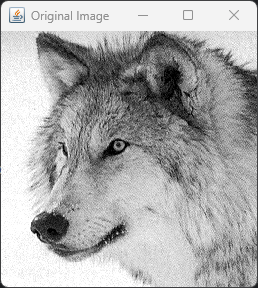
\includegraphics[width=0.49\columnwidth]{Figures/Week 1/W1-Wolf-Original.png}
            \caption{A screenshot of the original wolf image}
            \label{fig:wolf_image}
    \end{figure}
    
    A Fourier analysis is a mathematical technique which decomposes a waveform into its fundamental sinusoidal sub-components, representing the waveform in the frequency domain, opposed to the spatial domain. These Fourier components represent the frequency, amplitude and phase which make up the original signal. 
    Fourier analysis allows image processing (among other signal processes) to be performed. The sum of the sub-components is used to recreate the original waveform. 
    

    To begin, supporting Java classes were provided, they are: 
    \begin{itemize}
        \item DisplayDensity.java
        \item ReadPGM.java
        \item Display2dFT.java
        \item SimpleFT.java
    \end{itemize}
        
    'DisplayDensity.java' displays a greyscale image rendered from a 2D array.
    
    'ReadPGM.java' parses a .pgm file, 'Display2dFT.java' allows the Fourier Transform (FT) output to be represented graphically, using colour to represent imaginary number components. 'SimpleFT' is a skeleton program to code in.
    

    
    \subsection{Discrete Fourier Transform}
    To perform the DFT, the equation shown in \autoref{fig:equation-FT} must be implemented, C is a 2D array of length N.
    
    \begin{center}
        \begin{equation}
            C_{kl} = 1/N^2 \sum_{m=0}^{N-1} \sum_{n=0}^{N-1}\ X_{mn} . e^{-2\pi i(km+nl)/N}
            \label{fig:equation-FT}
        \end{equation}  
    \end{center}%Equation

    Implementation of the equation is shown in \autoref{fig:wolf-FT-code}. An array called 'X' stored the original .pgm data. The program decomposes the original frequencies into two arrays, this is because the process generates complex numbers. The imaginary component of the number is stored in 'CIm' while the real component is stored in 'CRe'. 
 
    \begin{figure}[H]
        \centering
        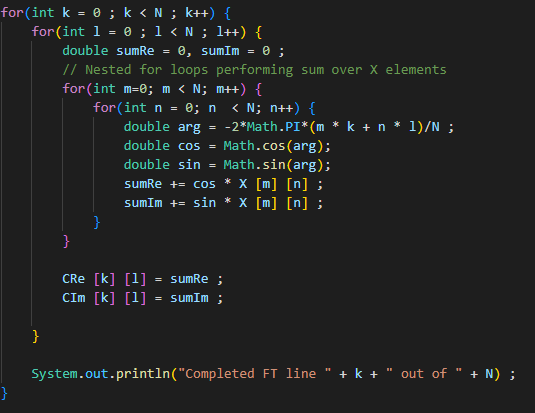
\includegraphics[width=1\columnwidth]{Figures/Week 1/W1-SimpleFT-Completed-For-Loop.png}
        \caption{A screenshot of the implementation of the Fourier Transform}
        \label{fig:wolf-FT-code}
    \end{figure}

    The graphical representation of the Fourier Analysis is shown in \autoref{fig:wolf-DFT}. 
    
    \begin{figure}[H]
        \centering
        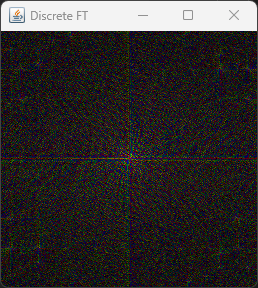
\includegraphics[width=0.49\columnwidth]{Figures/Week 1/W1-FT.png}
        \caption{A screenshot of the Discrete Fourier Transform graphical output}
        \label{fig:wolf-DFT}
    \end{figure}
    
    
    \subsection{Inverse Discrete Fourier Transform}
    The Inverse function is used to reconstruct the image from the frequency domain representation, by converting it back to a spatial domain. The equation \autoref{fig:equation-InverseFT} must be implemented to do this. 

    \begin{center}
        \begin{equation}
            X_{mn} = \sum_{k=0}^{N-1} \sum_{l=0}^{N-1}\ C_{kl} . e^{2\pi i(km+nl)/N}
            \label{fig:equation-InverseFT}
        \end{equation}  
        \end{center}
        
    The code of the implementation is shown in \autoref{fig:inverse-DFT-Code}.  Pixel value normalisation is performed to set pixel values to 'DisplayDensity' class can output the image correctly. 
        
        \begin{figure}[H]
            \centering
            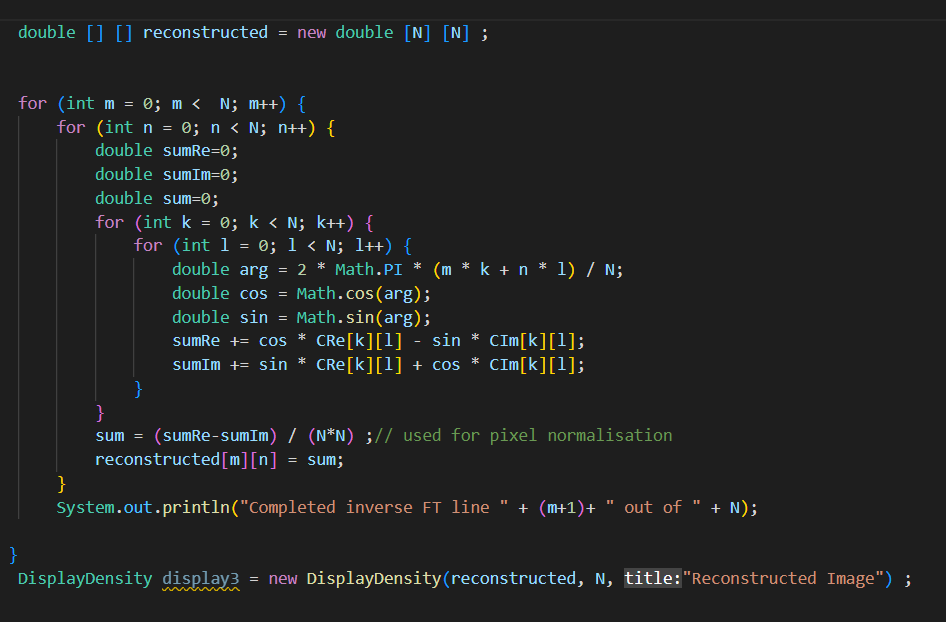
\includegraphics[width=0.9\columnwidth]{Figures/Week 1/W1-SimpleFT-InverseDFT-Implementation.png}
            \caption{A screenshot of the Java inverse DFT implementation}
            \label{fig:inverse-DFT-Code}
    \end{figure}

    All the graphical outputs of the program are shown in \autoref{fig:inverse-DFT-Images-Output}, the reconstructed image is on the right side. 
    
    \begin{figure}[H]
            \centering
            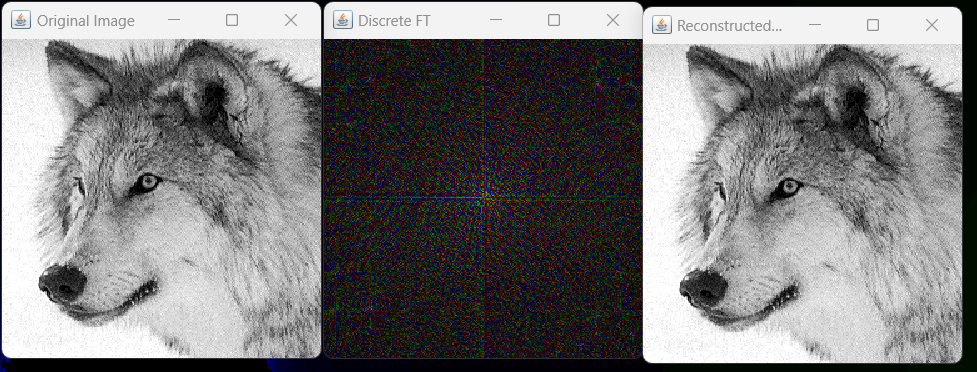
\includegraphics[width=0.8\columnwidth]{Figures/Week 1/W1-SimpleFT-InverseDFT-Graphical-Outputs.png}
            \caption{Graphical output of the program - inverse DFT reconstruction on the right side}
            \label{fig:inverse-DFT-Images-Output}
    \end{figure}

    While the outputted images are the same as the 'DisplayDensity' class essentially rounds values, the values in the new 'reconstructed' array deviate from the original 'X' array. This is due to the primitive double datatype in Java being a floating-point representation, causing some precision to be lost during calculations - this is called a floating-point error.
    
    \autoref{fig:Testing-Code} and \autoref{fig:Testing-Code-output} show the code and console output for detecting incorrectly reconstructed values. The 'reconstructed' values are close to the original.   
    
    \begin{figure}[H]
        \centering
        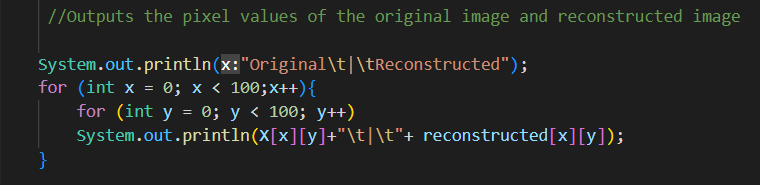
\includegraphics[width=1\columnwidth]{Figures/Week 1/W1-SimpleFT-InverseDFT-Test-1.0-code.png}
        \caption{A screenshot of the testing code}
        \label{fig:Testing-Code}
    \end{figure}
    \begin{figure}[H]
            \centering
            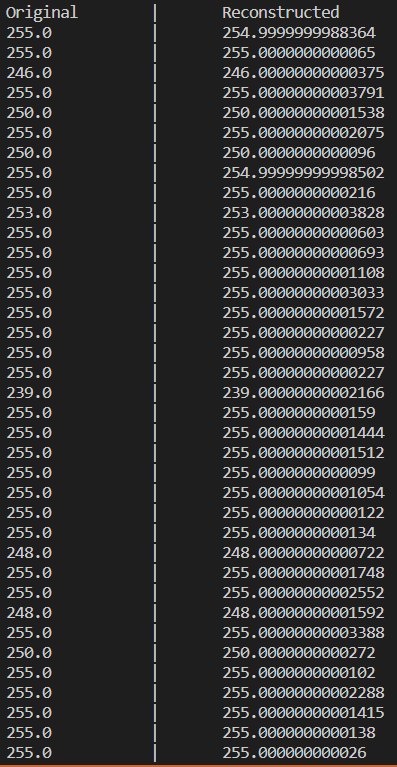
\includegraphics[width=.49\columnwidth]{Figures/Week 1/W1-SimpleFT-InverseDFT-Test-1.0-Output.png}
            \caption{A screenshot of the testing code output}
            \label{fig:Testing-Code-output}
        \end{figure}

    \autoref{fig:floating-Point-Fix}, \autoref{fig:floating-Point-Fixed-test} and \autoref{fig:floating-Point-Fixed-CLI-Output} shows that the error can be completely removed by rounding each reconstructed value to the nearest integer.
    \newpage
    \begin{figure}[H]
        \centering
        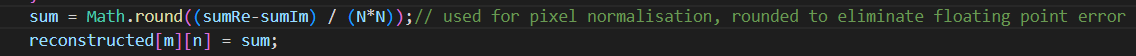
\includegraphics[width=1\columnwidth]{Figures/Week 1/W1-SimpleFT-InverseDFT-Floating-Point-Fix.png}
        \caption{A screenshot of code to fix floating point error}
        \label{fig:floating-Point-Fix}
    \end{figure}
    \begin{figure}[H]
            \centering
            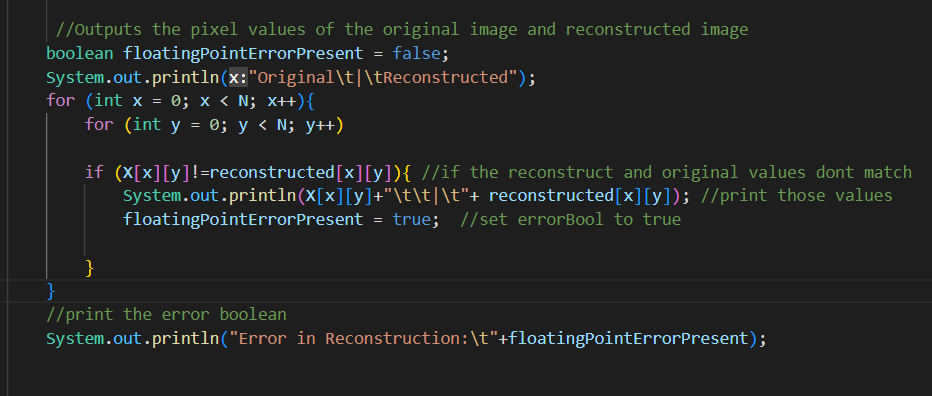
\includegraphics[width=1\columnwidth]{Figures/Week 1/W1-SimpleFT-InverseDFT-Test-2.0-code.png}
            \caption{A screenshot of code to test the floating point error fix}
            \label{fig:floating-Point-Fixed-test}
        \end{figure}   
    \begin{figure}[H]
            \centering
            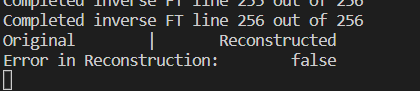
\includegraphics[width=0.8\columnwidth]{Figures/Week 1/W1-SimpleFT-InverseDFT-Test-2.0-CLI-Output.png}
            \caption{A screenshot of console output showing floating point error test has passed}
            \label{fig:floating-Point-Fixed-CLI-Output}
        \end{figure}
        
   
    \newpage
    \subsection{Filtering}
    Now that the data is in the frequency domain, performing filtering operations are simple. 
    
    \subsubsection{Low Pass Filter}
    A low pass filter removes frequencies above a cutoff value allowing low frequencies to pass through. In this instance, the cutoff was set to $N/8$ or $256/8$. \autoref{fig:Low-Pass-Filter-code} shows that any values greater than the cutoff are set to $0$. The absolute value of each input value is used to remove the sign from the number, allowing the conditional statements to function correctly. 
    
    \begin{figure}[H]
        \centering
        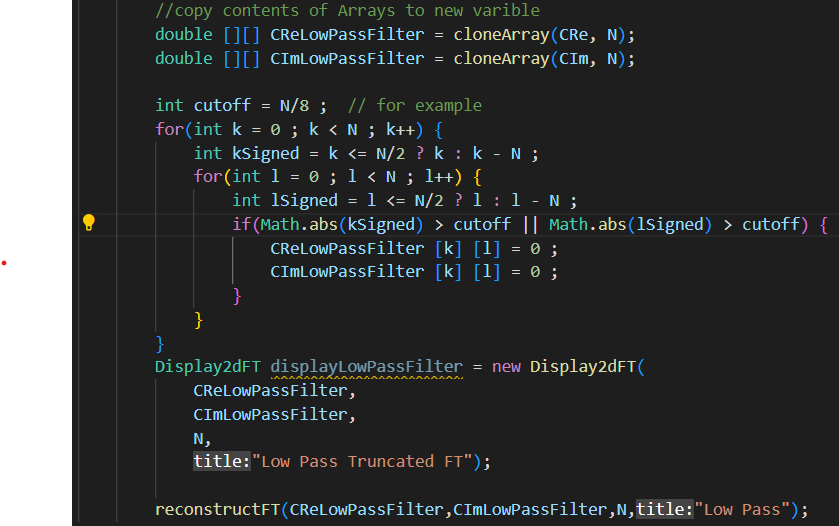
\includegraphics[width=0.8\columnwidth]{Figures/Week 1/W1-Low-Pass-Code.png}
        \caption{Screenshot of FT low pass filter code}
        \label{fig:Low-Pass-Filter-code}
      \end{figure}

    \autoref{fig:Low-Pass-Filter-Truncated} shows the truncated FT graphic, note the large black area which represents the removed frequencies. In \autoref{fig:Low-Pass-Filter-Image}, a lot of detail is clearly missing from the image.
    \begin{figure}[H]
        \centering
        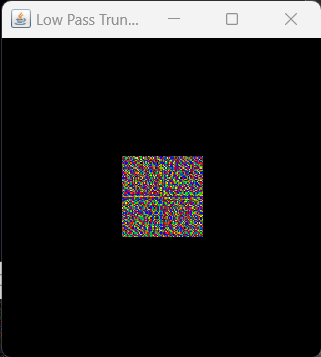
\includegraphics[width=0.49\columnwidth]{Figures/Week 1/W1-Low-Pass-Truncated.png}
        \caption{Screenshot of the low pass filter truncated FT graphical output}
        \label{fig:Low-Pass-Filter-Truncated}
      \end{figure}
    \begin{figure}[H]
        \centering
        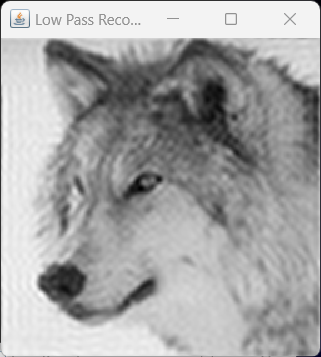
\includegraphics[width=0.49\columnwidth]{Figures/Week 1/W1-Low-Pass-Reconstructed.png}
        \caption{Screenshot of the low pass filter reconstructed image output}
        \label{fig:Low-Pass-Filter-Image}
      \end{figure}

    
    \newpage    
    \subsubsection{High Pass Filter}
    Next, a high pass filter was implemented. This filter does the opposite of the previous one and removes frequencies below a cutoff value. \autoref{fig:High-Pass-Filter-code} shows the implementation is similar to the low pass filter. The cutoff value was set to $N/128$ and again sets values to $0$. 
    
    \begin{figure}[H]
        \centering
        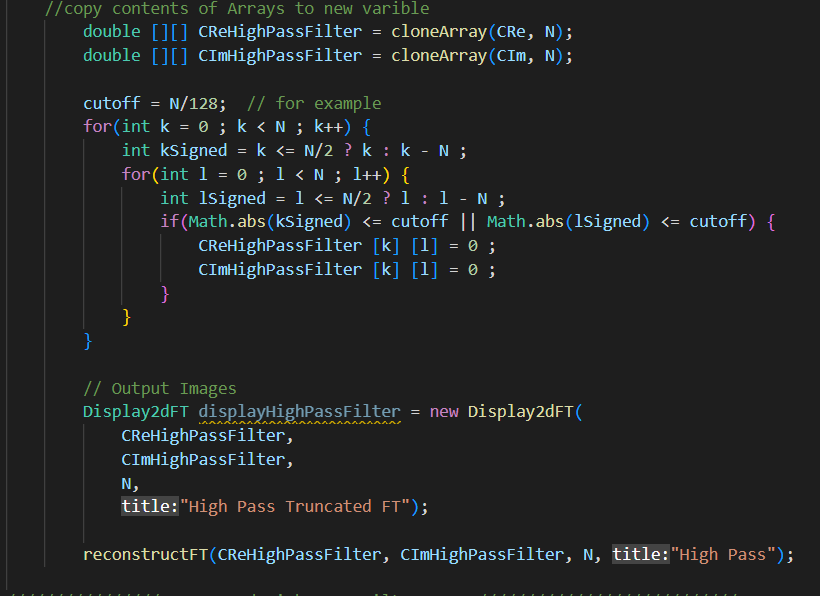
\includegraphics[width=.9\columnwidth]{Figures/Week 1/W1-High-Pass-Code.png}
        \caption{Screenshot of FT high pass filter code}
        \label{fig:High-Pass-Filter-code}
    \end{figure}
    

    \autoref{fig:High-Pass-Filter-Truncated} shows the truncated FT and \autoref{fig:High-Pass-Filter-Image} shows the final image.
      \begin{figure}[H]
        \centering
        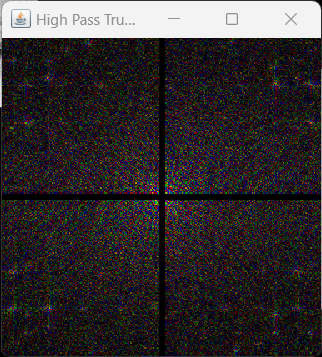
\includegraphics[width=0.49\columnwidth]{Figures/Week 1/W1-High-Pass-Truncated.png}
        \caption{Screenshot of the high pass filter truncated FT graphical output}
        \label{fig:High-Pass-Filter-Truncated}
      \end{figure}

      \begin{figure}[H]
        \centering
        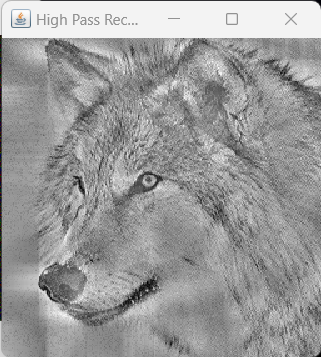
\includegraphics[width=0.49\columnwidth]{Figures/Week 1/W1-High-Pass-Reconstructed.png}
        \caption{Screenshot of the high pass filter reconstructed image output}
        \label{fig:High-Pass-Filter-Image}
      \end{figure}

      \subsubsection{Combined Filters}
      Finally, \autoref{fig:Combined-Filters} shows both filters combined. This has caused some detail in the image to be lost and the visible noise to be reduced, however, new artefacts have been produced.
        \begin{figure}[H] 
            \centering
            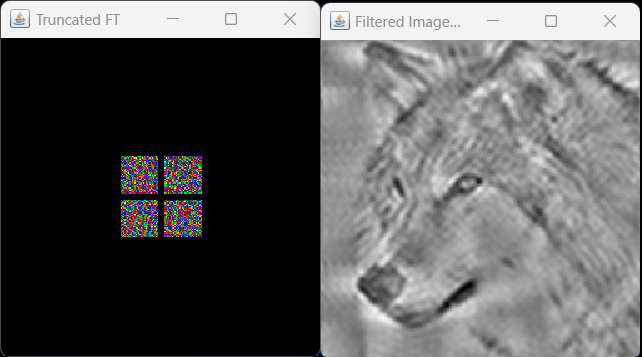
\includegraphics[width=0.8\columnwidth]{Figures/Week 1/W1-Both-Filters.png}
            \caption{Screenshot of the graphical output when filters are combined}
            \label{fig:Combined-Filters}
        \end{figure}



\newpage
\section{Lab 2 - Fast Fourier Transform}
This week, an FFT was implemented and benchmarked against the previous FT implementation. 

The time complexity for the original FT is $O(N^2)$, and the time complexity for the FFT is $O(N log N)$.
This is achieved by taking advantage of symmetries which occur in the calculation, reducing the total number of calculations required. These symmetries, or twiddle factors, are coefficients which reoccur on every even or every odd index. It is by reusing the calculated twiddle factors that allow the FT to be completed in less time. This is the approach taken in the  Cooley–Tukey FFT algorithm using recursion to divide the problem.

\subsection{2D FFT Implementation}

Java support classes 'FFT.java' and 'FFTImageFiltering.java' was provided. The first class contains code to perform a one-dimensional FFT and its inverse, the latter is a skeleton program to code in. 

To implement a 2D FFT using the fft1d method from the 'FFT' class, a helper function was implemented to transpose the 2D arrays. This is shown in \autoref{fig:transpose-code}. 

    \begin{figure}[H] 
        \centering
        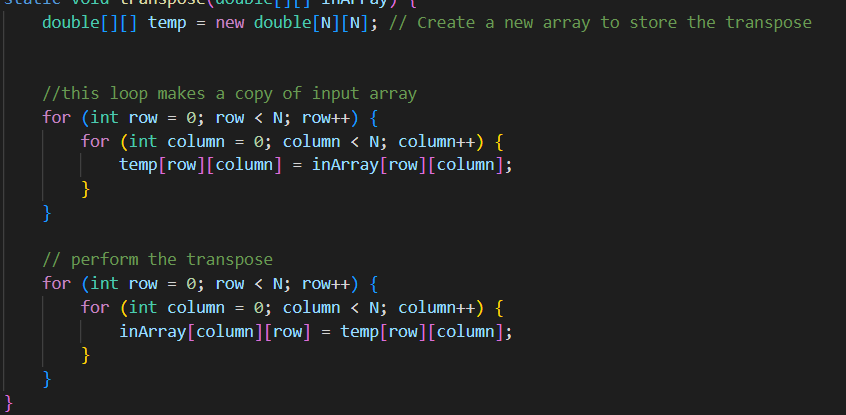
\includegraphics[width=0.8\columnwidth]{Figures/Week 2/Transpose Implementation.png}
        \caption{Screenshot of Java code showing the transpose implementation}
        \label{fig:transpose-code}
    \end{figure}

\autoref{fig:2dFFT-code} shows the implementation of 2D-FFT from the 1D-FFT, a loop iterates over the input arrays 'CRe' and 'CIm', performing an FFT on each row before transposing both arrays and repeating once again. This ensures that the FFT is applied to both axes of the input arrays.

    \begin{figure}[H] 
        \centering
        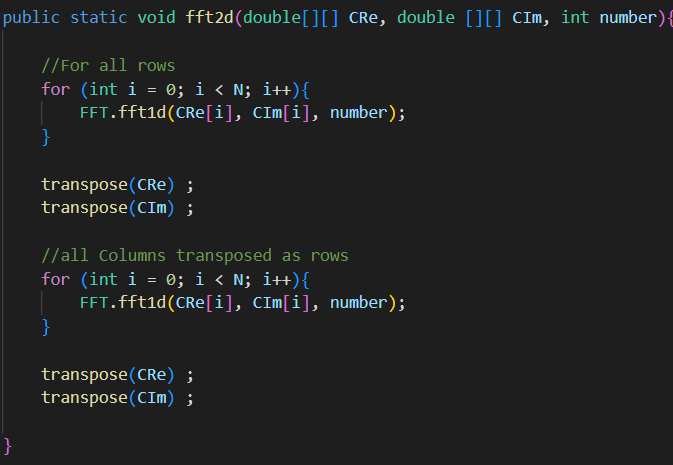
\includegraphics[width=0.8\columnwidth]{Figures/Week 2/2dFFT Implementation.png}
        \caption{Screenshot of Java code showing the 2D FFT function implementation}
        \label{fig:2dFFT-code}
    \end{figure}

\subsection{Benchmarking}


Benchmarking code was added to both programs to compare run times. \autoref{fig:bench-code-start} and \autoref{fig:bench-code-end} show the benchmarking code implementation and \autoref{fig:SimpleFT-Bench} shows the console output when run.


    \begin{figure}[H] 
        \centering
        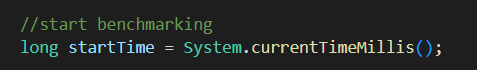
\includegraphics[width=0.8\columnwidth]{Figures/Week 2/Bench code Start.png}
        \caption{Screenshot of Java Benchmarking code at start of main}
        \label{fig:bench-code-start}
    \end{figure}
    \begin{figure}[H] 
        \centering
        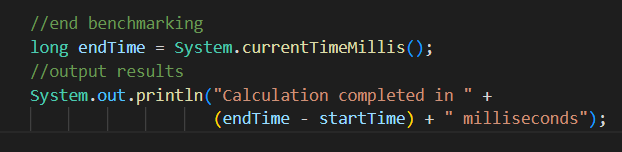
\includegraphics[width=0.8\columnwidth]{Figures/Week 2/Bench code end.png}
        \caption{Screenshot of Java Benchmarking code at end of main}
        \label{fig:bench-code-end}
    \end{figure}
    \begin{figure}[H] 
        \centering
        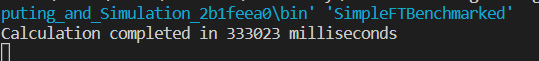
\includegraphics[width=0.8\columnwidth]{Figures/Week 2/SimpleFT Bench.png}
        \caption{Screenshot of the Console output from SimpleFT Benchmarking code}
        \label{fig:SimpleFT-Bench}
    \end{figure}

    Each program was run 3 times the results from the benchmarking is shown in \autoref{tab:W2-bench-results-table}. 

    \begin{table}[htbp]
      \centering
      \resizebox{1\columnwidth}{!}{\begin{tabular}{|c|c|c|c|c|}
         \hline
        \textbf{Run Number} & \textbf{SimpleFT (ms)} & \textbf{SimpleFT With Filters (ms)} & \textbf{Fast FT (ms)} & \textbf{Fast FT With filters (ms)}\\
        \hline
        Run 1 & 333023 & 673758 & 816 & 789\\
        \hline
        Run 2 & 315853 & 590674 & 600 & 971\\
        \hline
        Run 3 & 297395 & 524380 & 668 & 954\\
        \hline
        Mean Average & 315424 & 596271 & 695 & 905\\
        \hline
      \end{tabular}}
      \caption{Lab 2 FFT Benchmarking Results}
      \label{tab:W2-bench-results-table}
    \end{table}
    
    \begin{figure}[H] 
        \centering
        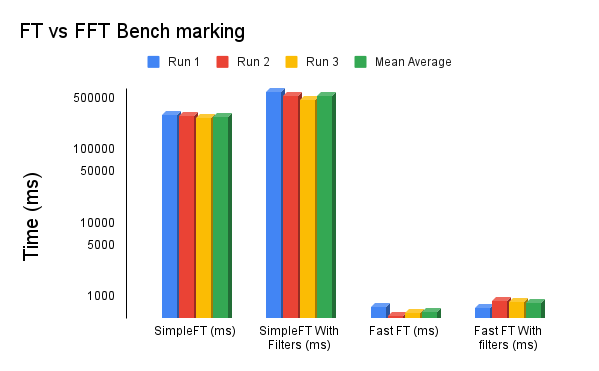
\includegraphics[width=0.8\columnwidth]{Figures/Week 2/FT vs FFT Bench marking.png}
        \caption{Screenshot of FFT vs FT benchmark results graph}
        \label{fig:W2-Benchmarking-Graph}
    \end{figure}

    In all cases, the FFT outperformed the FT by a large margin. This is illustrated in \autoref{fig:W2-Benchmarking-Graph}, showing that the FFT programs has a much faster run time than the previous implementations. 
    
    The mean average of the three runs is used in the following calculations. The FFT program with no filtering allowed for a speedup of  $315424 / 695 = 53.85$.The programs with filtering allowed for a speedup of $596271 / 905 = 658.86$. In both cases, the programs ran much faster when using the FFT implementation.

    Overall the FFT is a far better approach than the naive implementation as it can perform an FT in a fraction of the time.
    
\newpage
\section{Lab 3 - CT Scanner}

This lab explores the computations required for a CT scanner, an FT and filtering is applied to a sinogram to recover visual data. A Radon Transform (RT) (\textcite{4307775} was implemented to calculate the densities for the back-projected sinogram. 

An RT is similar to an FT, however, it produces a set of line integrals or projections which capture the distribution of linear structures within the image. An RT takes two parameters angle '$\theta$' and offset 'r', where '$\theta$' is the orientation angle of the detector assembly and 'r' is the offset of a single detector to the assembly. The transform differs from an FT as it outputs a set of line integrals that capture the distribution of linear structures within the image, rather than frequency information.

Two classes were supplied, 'DisplaySinogramFT.java' rendered the Sinogram-FT as an image and 'Sinogram.java' contains a skeleton program which includes the initial body slice model. It outputs the initial model and calculated sinogram before outputting a back-projected sinogram. The back-projected image contains little detail, this is shown on the right side of \autoref{fig:W3-initial-output}. The back-projected sinogram image is simply an inverse RT.

The initial source model is the 'Shepp Logan Phantom' \textcite{6499235}, which is made of a series of ellipses representing different densities. The code performs an RT on the model densities to produce the Sinogram, the inversion of this transform will produce the final image. 


\begin{figure}[H] 
    \centering
    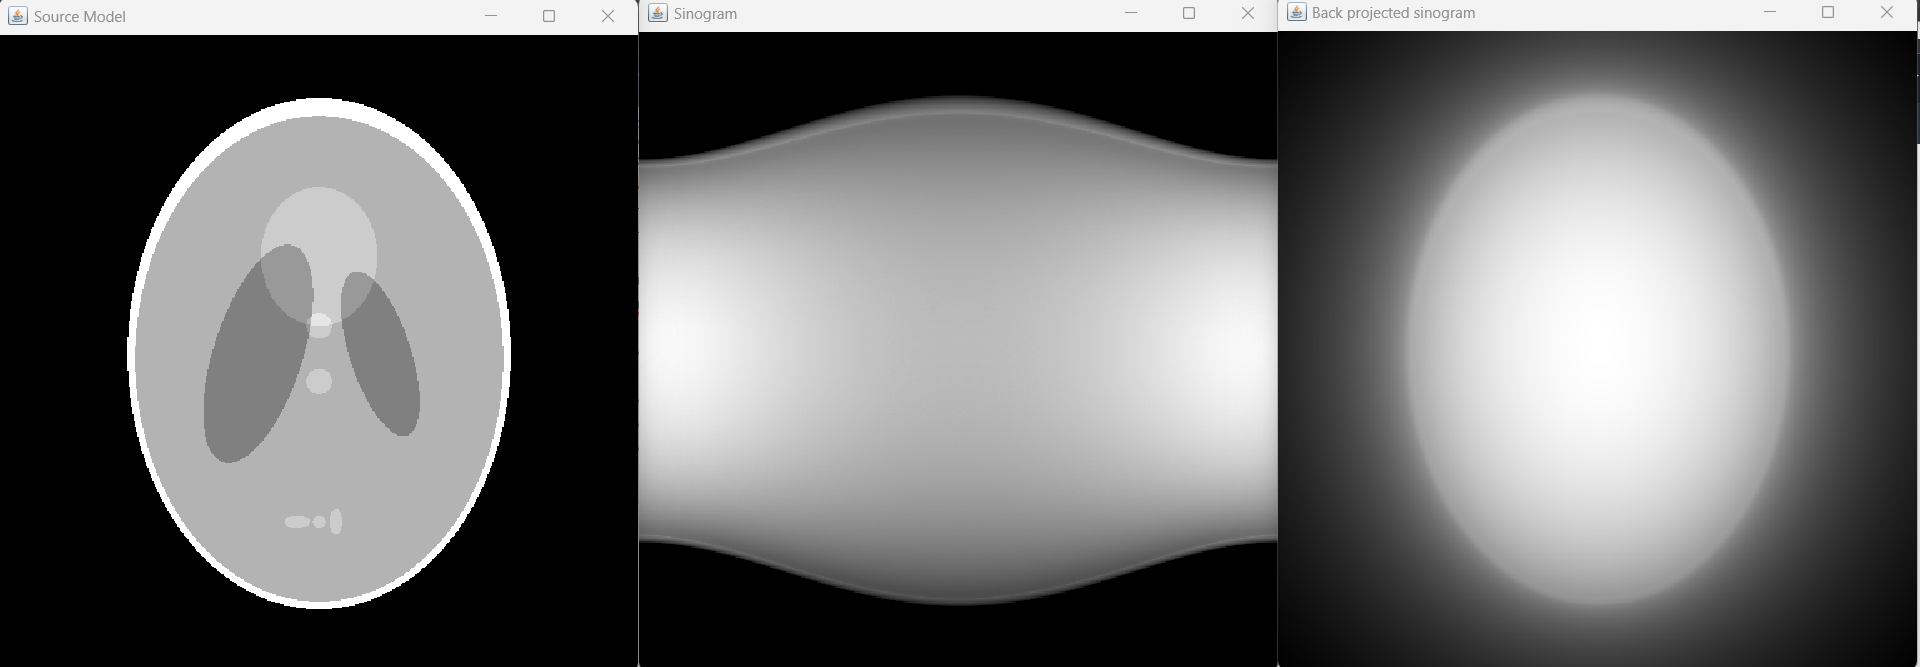
\includegraphics[width=0.9\columnwidth]{Figures/Week 3/initial-graphics.png}
    \caption{Screenshot of the graphical output of the initial Sinogram.java}
    \label{fig:W3-initial-output}
\end{figure}


\subsection{Applying an FFT}
Filtering the sinogram is required to make details more visible in the back-projected image. In order to perform filtering, a complex FFT is performed over \(\theta\) on the sinogram, the graphical output of this FFT is shown in \autoref{fig:W3-initial-FT}. Implementation code is shown in \autoref{fig:W3-initial-FT-code}.

\begin{figure}[H] 
    \centering
    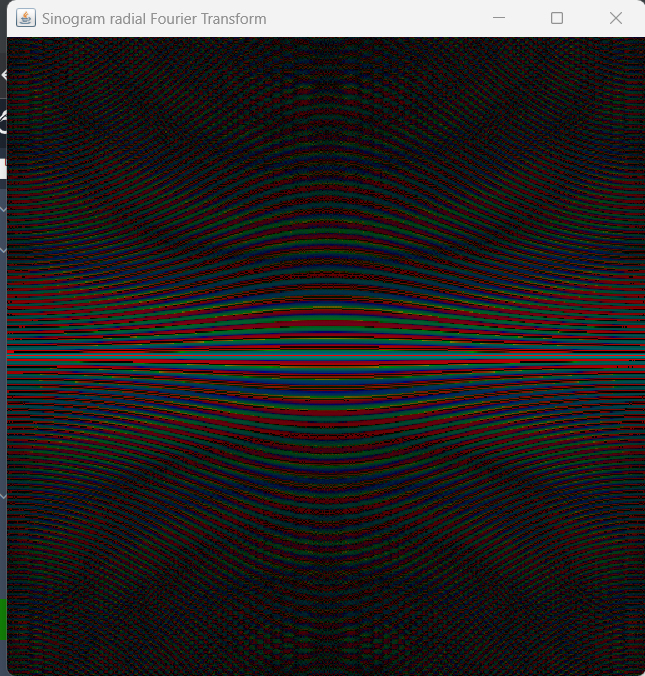
\includegraphics[width=0.49\columnwidth]{Figures/Week 3/initial-FFTpng.png}
    \caption{Screenshot of the graphical output of the initial Sinogram Fourier Transform}
    \label{fig:W3-initial-FT}
\end{figure}
\begin{figure}[H] 
    \centering
    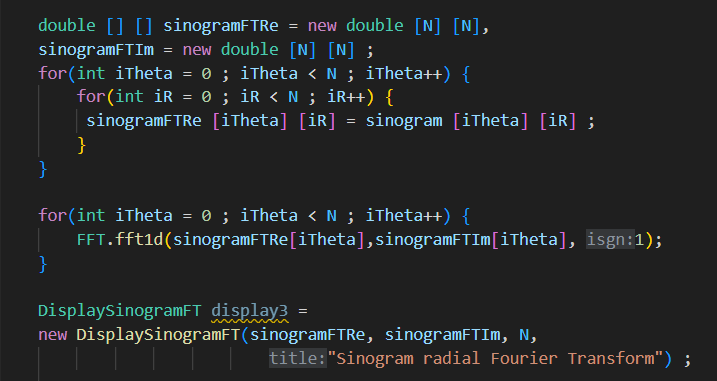
\includegraphics[width=0.9\columnwidth]{Figures/Week 3/initial-FFT-code.png}
    \caption{Screenshot of the code performing the Sinogram Fourier Transform}
    \label{fig:W3-initial-FT-code}
\end{figure}




\subsection{Applying a Simple Ramp Filter}
Next, the filter must be applied to the Fourier Transform data. A simple Ramp filter has been implemented. A ramp filter is a high-pass filter which reduces low frequencies to decrease blurring. The code is shown in \autoref{fig:W3-ramp-code}. For each element, the code generates a $|K|$ value which is then multiplied by both the real and imaginary numerical components of the Fourier Transform.

The value of 'kSigned' is set to 'iK' if the value is $iK <= N/2$, otherwise, the value is set to $iK-N$.

\begin{figure}[H] 
    \centering
    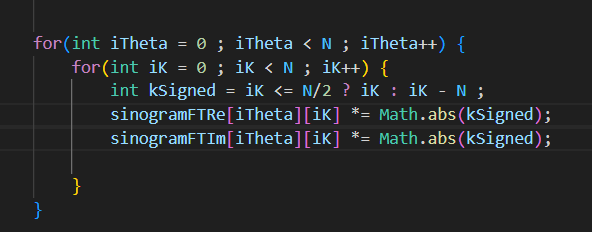
\includegraphics[width=0.9\columnwidth]{Figures/Week 3/ramp-filter-code.png}
    \caption{Screenshot of the code performing the Ramp filter}
    \label{fig:W3-ramp-code}
\end{figure}

The next step is to rebuild the Sinogram by performing an inverse Fourier Transform over \(\theta\), code is shown in \autoref{fig:W3-inverse-code}.

\begin{figure}[H] 
    \centering
    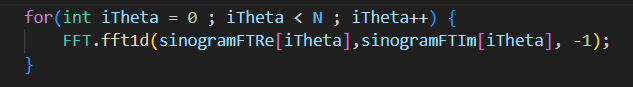
\includegraphics[width=0.9\columnwidth]{Figures/Week 3/inverse-FT.png}
    \caption{Screenshot of the code performing Inverse FT }
    \label{fig:W3-inverse-code}
\end{figure}

The filtered sinogram is shown in \autoref{fig:W3-filtered-sin}.
\begin{figure}[H] 
    \centering
    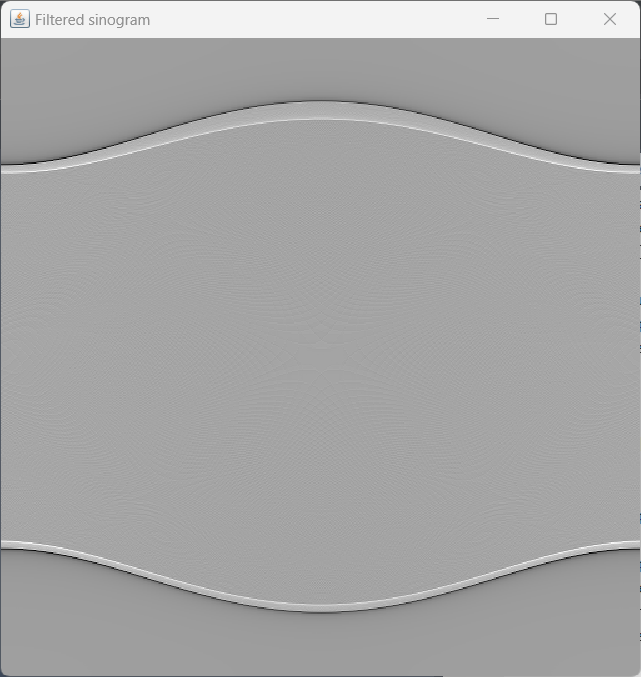
\includegraphics[width=0.9\columnwidth]{Figures/Week 3/filtered-sinorgram.png}
    \caption{Screenshot of the graphical output for the filtered sinogram}
    \label{fig:W3-filtered-sin}
\end{figure}

To output the filtered back-projected image, a back-projection operation is performed on the sinogram before the values are normalised. The new image is then drawn. This is shown in \autoref{fig:W3-filtered-back-image}. More detail is visible in the back-projected image, however, a lot of noise has been introduced. To reduce this noise, further filtering is required.
    
\begin{figure}[H] 
    \centering
    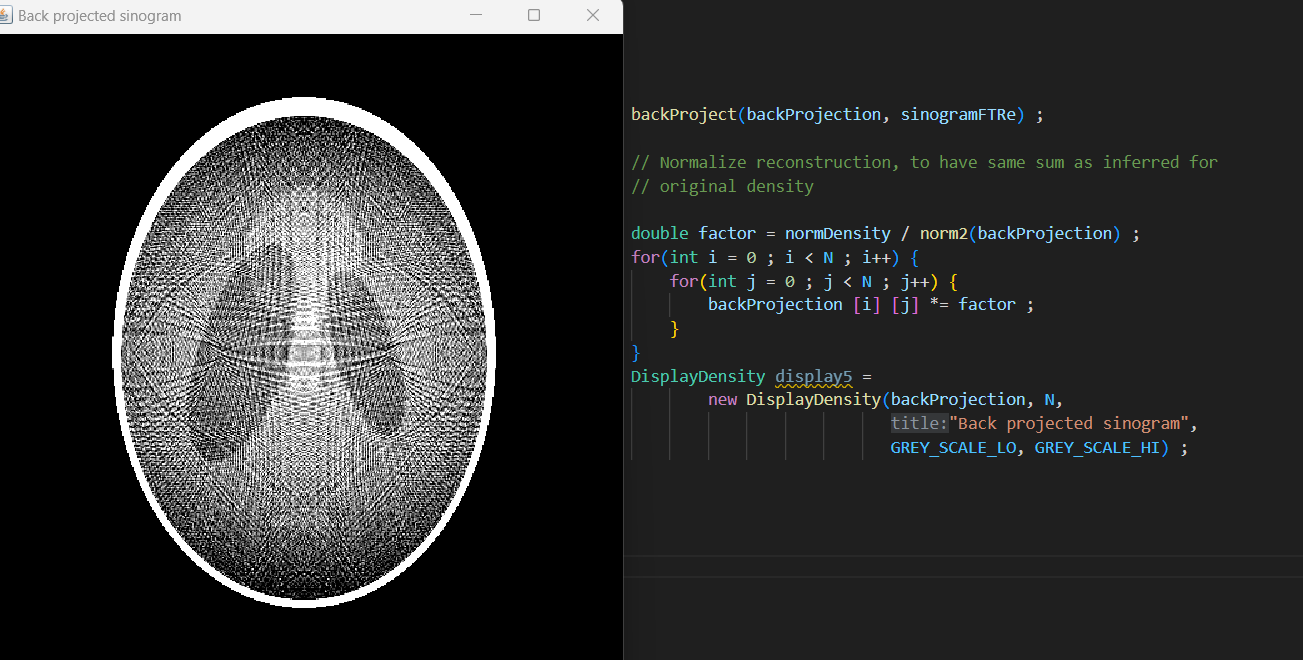
\includegraphics[width=1\columnwidth]{Figures/Week 3/filtered-back-projection.png}
    \caption{Screenshot the filtered back-projected sinogram}
    \label{fig:W3-filtered-back-image}
\end{figure}


\subsection{Applying a Ramp Filter with Cutoffs}
The previous filter was altered to make use of a cutoff value, and an integer variable 'CUTOFF' was created. This stores the value of: '$N / Value$'. If the '$|K|$' value is greater than this CutOff, the Fourier Component is set to '0'. The code for this implementation is shown in \autoref{fig:W3-filter-with-cutoff-code}.

\begin{figure}[H] 
    \centering
    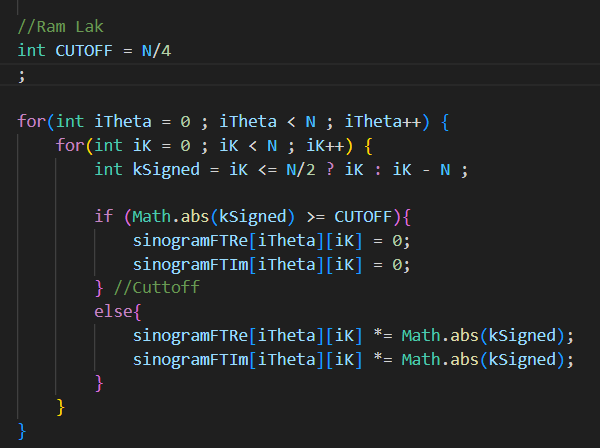
\includegraphics[width=1\columnwidth]{Figures/Week 3/Filter-with-cuttoff-code.png}
    \caption{Screenshot of the Java code performing filtering with cutoff value}
    \label{fig:W3-filter-with-cutoff-code}
\end{figure}


The program was run with $N/4$ and $N/16$, the back-projected images do have slightly reduced noise. \autoref{fig:W3-many-filters} shows the back-projected images made using a Ramp filter with no CUTOFF (left), with CUTOFF=N/4 (centre) and CUTOFF=N/16 (right).  



\begin{figure}[H] 
    \centering
    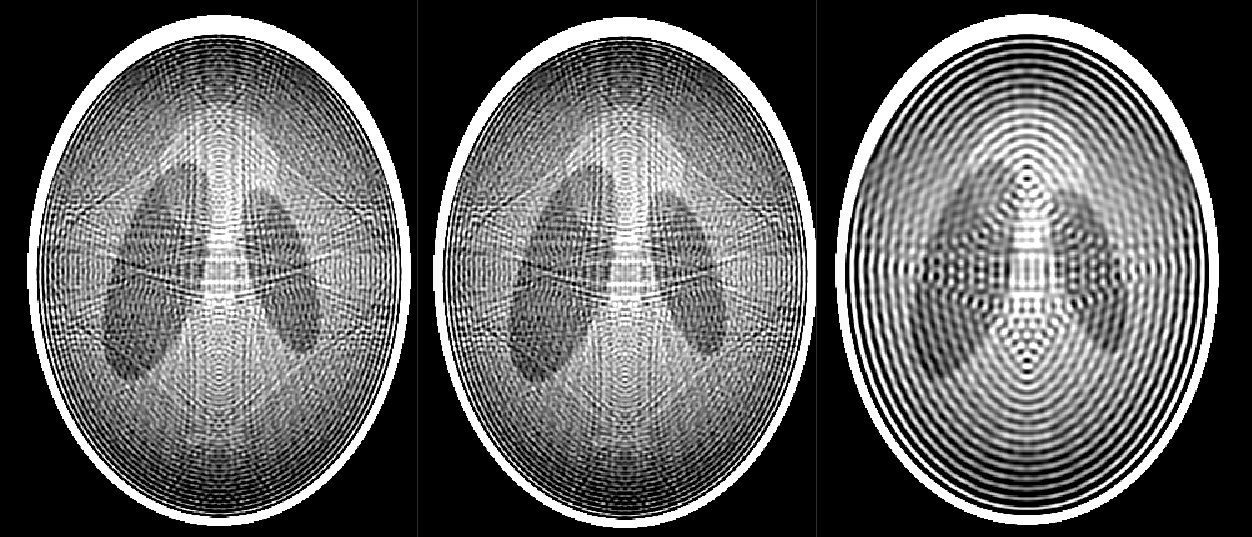
\includegraphics[width=1\columnwidth]{Figures/Week 3/filtered-images-ramp-N-4-N-16.png}
    \caption{Screenshot of back project images with filters applied}
    \label{fig:W3-many-filters}
\end{figure}


\newpage
\subsection{Applying Low Pass Cosine Filter}

Next, a low-pass Cosine Filter was applied. The filter takes a similar approach to the previous high-pass filter but applies the following equation. \(|K|  cos(\pi K /(2  *  CUTOFF))\).

Implementation is shown in \autoref{fig:W3-cos-filter-code}. 

\begin{figure}[H] 
    \centering
    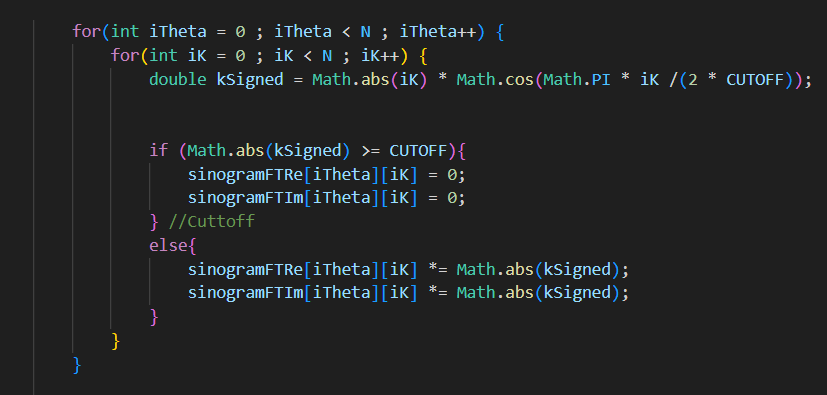
\includegraphics[width=1\columnwidth]{Figures/Week 3/filter-cos-codfe.png}
    \caption{Screenshot of the cosine filter code}
    \label{fig:W3-cos-filter-code}
\end{figure}

\autoref{fig:W3-cos-filter-image} shows the image when CUTOFF=$N/4$. The image has little noise removed,
\autoref{fig:W3-cos-filter-image-n-8} shows the image when CUTOFF=$N/8$, the image is now missing a lot of detail compared to the results of the standard ramp filter. 
\begin{figure}[H] 
    \centering
    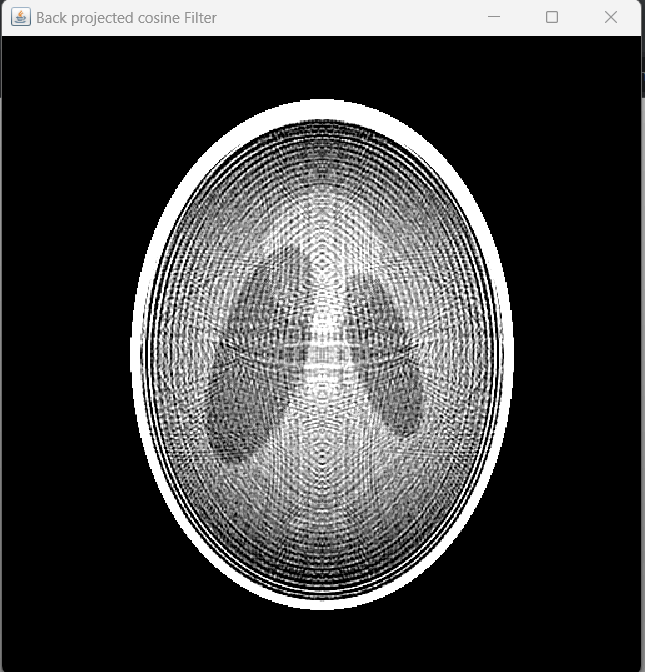
\includegraphics[width=0.49\columnwidth]{Figures/Week 3/filter-cos-image.png}
    \caption{Screenshot of the cosine filter image Cutoff=N/4}
    \label{fig:W3-cos-filter-image}
\end{figure}
\begin{figure}[H] 
    \centering
    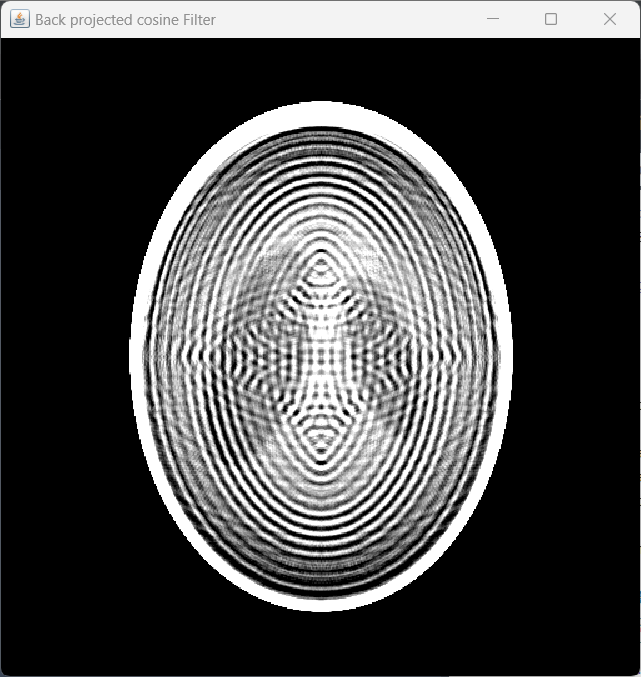
\includegraphics[width=0.49\columnwidth]{Figures/Week 3/filter-cos-image-N-8.png}
    \caption{Screenshot of the cosine filter image Cutoff=N/8}
    \label{fig:W3-cos-filter-image-n-8}
\end{figure}


\newpage
\section{Lab 4 - Radio Interferometry}

Radio Interferometry is a technique used in Astrophotography which makes use of multiple radio telescopes spread over a large area to gather data. The data is then processed afterwards to produce an image.

These are sometimes referred to as software telescopes, they require a great deal of processing to combine signals to produce an image. Two or more signals are combined constructively or destructively (depending on their relative phase) to accomplish this. These telescopes are spread over a large area and connected through an interferometric array \textcite{Borcea_2005}, radiowaves emitted by celestial objects are detected and stored for later processing. To 'aim' at an object, time delays are inserted into all the signals causing signals from a single direction to be in phase with each other.

Visibilities must be calculated to produce an image, visibility is a correlation function between signals arriving in two receivers. To calculate the visibility, the signals are first multiplied together and averaged over a fixed amount of time. This allows the cosine correlator $Rc$ to be obtained. A 90\textdegree phase shift is introduced to a signal. The signals are multiplied and averaged over time to obtain the Sine correlator $Rs$.

The visibility between the antennas is $V =Rc - iRs$

The sky intensity is the amount of radiowaves received from a particular direction in the sky. If $l, m$ are direction cosines relating to a position in the sky from a fixed origin, then the sky intensity function of position is denoted as $I(l,m)$.

If $(u, v)$ are the displacement of two telescopes, then the sky intensity can be calculated using the van Cittert-Zernike \autoref{eq:van-Cittert-Zernike}, this is an FT.

\begin{equation}
V(u, v) \propto \sum_{l} \sum_{m} I(l, m) \cdot e^{-2\pi i(ul + vm)}
\label{eq:van-Cittert-Zernike}
\end{equation}

To recover the image we perform an inverse FT 

\begin{equation}
I(l, m) \propto \sum_{u=-\infty}^{+\infty} \sum_{v=-\infty}^{+\infty} V(u, v) \cdot e^{2\pi i(ul + vm)}
\label{eq:van-Cittert-Zernike-inverse}
\end{equation}

This process can be used to create a 'dirty image', in industry, extra processing would be performed on the data to improve the image quality and accuracy. To gather extra data points, multiple telescopes are used in addition to sampling the sky at different times when the telescopes are in a different position (because of the planet's rotation).

A class 'Imaging.java' was provided, it processes a LOFAR data set to produce a point map and an image. \autoref{fig:W4-spiral-being-made} shows points being plotted as the program ran, on the left is at the beginning, a swirl can be seen  as time goes on. Once the program loop has run, \autoref{fig:W4-image-final-swirl} is drawn. It shows the swirls calculated, \autoref{fig:W4-grey-scale} shows a greyscale image of this.  


\begin{figure}[H] 
    \centering
    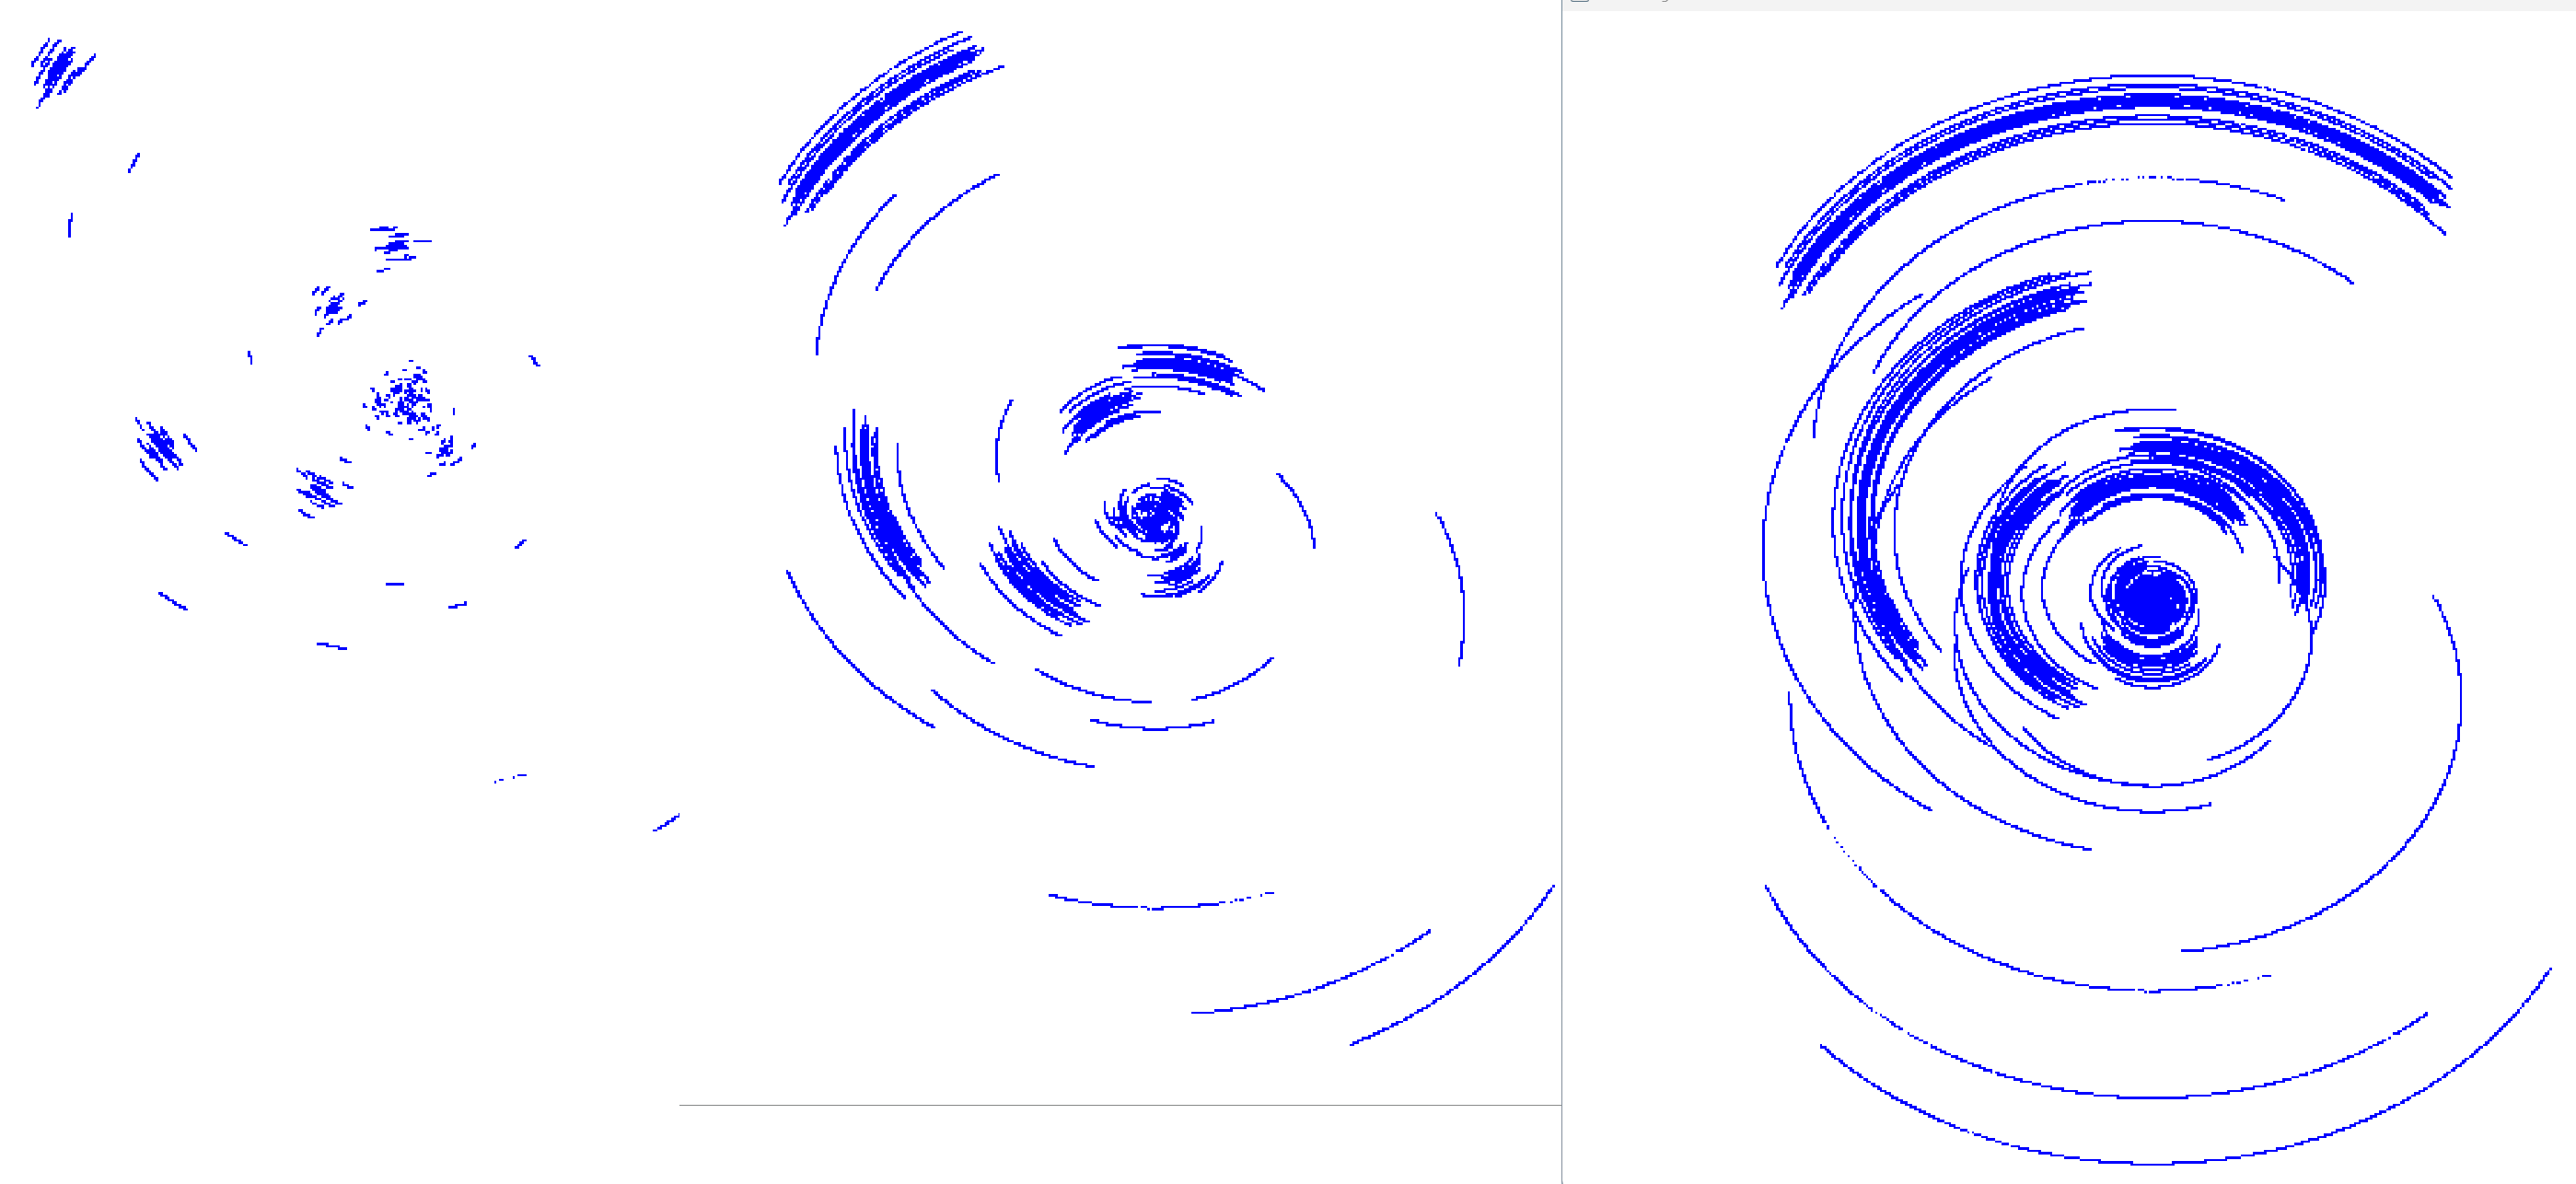
\includegraphics[width=0.49\columnwidth]{Figures/Week 4/spiral being made.png}
    \caption{Screenshot of the graphical output from Imaging.java }
    \label{fig:W4-spiral-being-made}
\end{figure}
\begin{figure}[H] 
    \centering
    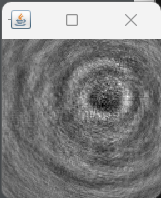
\includegraphics[width=0.49\columnwidth]{Figures/Week 4/Grey-scale-img.png}
    \caption{Screenshot of the greyscale graphical output Imaging.java}
    \label{fig:W4-grey-scale}
\end{figure}

\begin{figure}[H] 
    \centering
    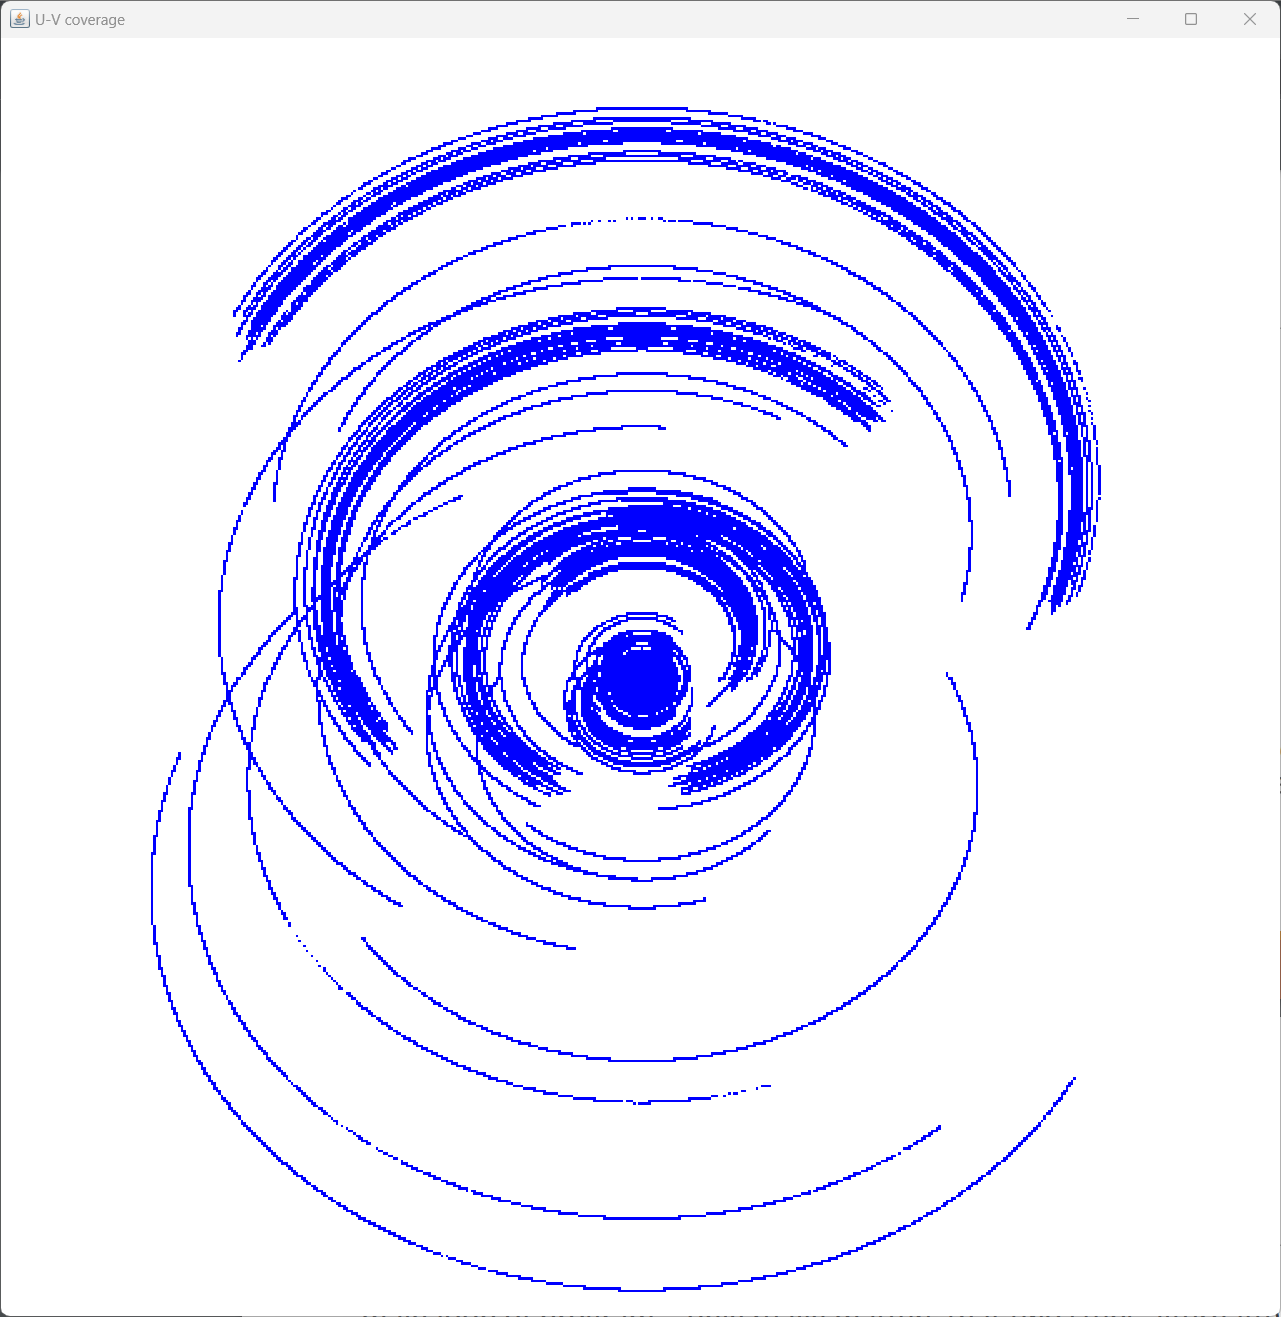
\includegraphics[width=0.49\columnwidth]{Figures/Week 4/Final swirls img.png}
    \caption{Screenshot of the final graphical output of Imaging.java}
    \label{fig:W4-image-final-swirl}
\end{figure}

\newpage
\section{Lab 5 - Lattice gas models}
Lattice gas models (LGM) are explored in this lab. An LGM is a cellular automata (CA) used to simulate fluid dynamics on a lattice grid.
Navier-Stokes is a differential equation which describes fluid flow, it is derived from Newton's second law of motion and can be used to accurately simulate particle collision. LGMs can be used to approximate this equation.


\subsection{HPP}
A basic Hard-Particle Packing (HPP) model was implemented, each cell on the lattice contains a state of a particle which represents one of four directions the particle is travelling in.

There are two steps in the HPP model which are run in a loop. In each iteration, the 'streaming' step simply moves a particle one cell in the direction it has inertia in (defined by its state) and the 'collision' step updates the particle state if there is a collision. In a collision, each particle's direction is set to be perpendicular to its previous direction. Each iteration represents one 'step' in time

A skeleton program called 'HPP.java' was provided. The implementation of the streaming and collision step is shown in \autoref{fig:W5-streaming-code} and \autoref{fig:W5-collision-step-code} respectively.


\begin{figure}[H] 
    \centering
    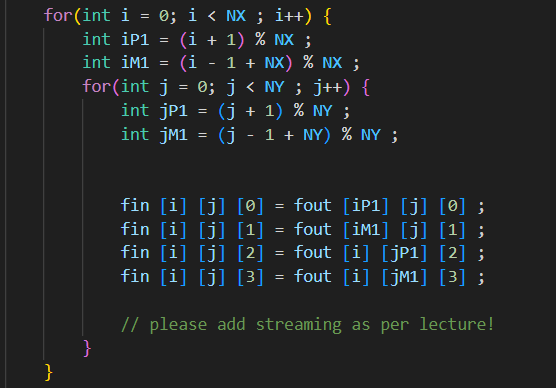
\includegraphics[width=0.59\columnwidth]{Figures/Week 5/HPP Streaming Step code.png}
    \caption{Screenshot of the HPP Streaming step code}
    \label{fig:W5-streaming-code}
\end{figure}

\begin{figure}[H] 
    \centering
    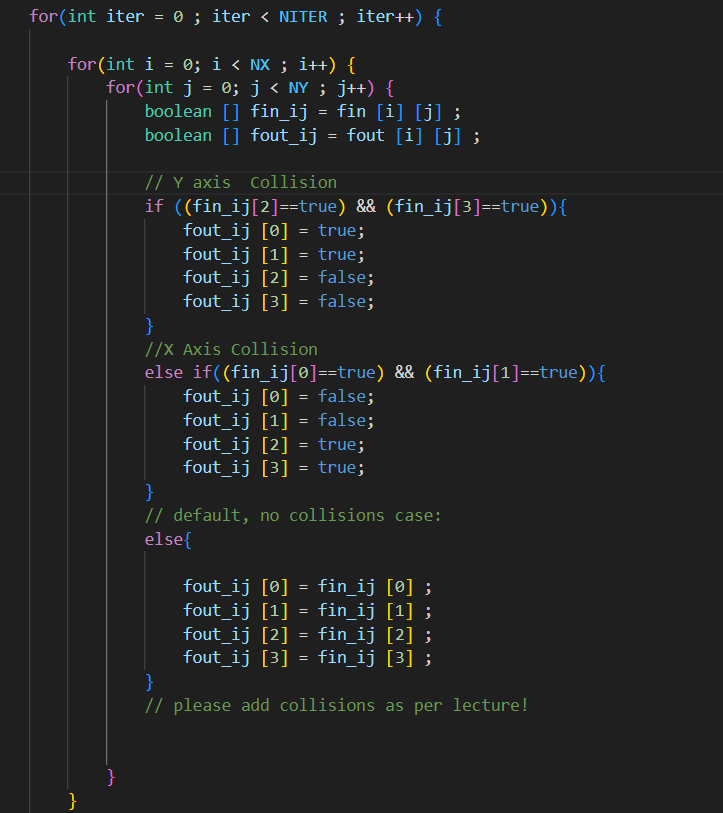
\includegraphics[width=0.59\columnwidth]{Figures/Week 5/HPP Collision Step code.png}
    \caption{Screenshot of the HPP Collision step code}
    \label{fig:W5-collision-step-code}
\end{figure}

The code was tested to ensure collisions were working using two particles in both axis directions. \autoref{fig:W5-hpp-before} and \autoref{fig:W5-hpp-after} show multiple particles before and after collision respectively.
\begin{figure}[H] 
    \centering
    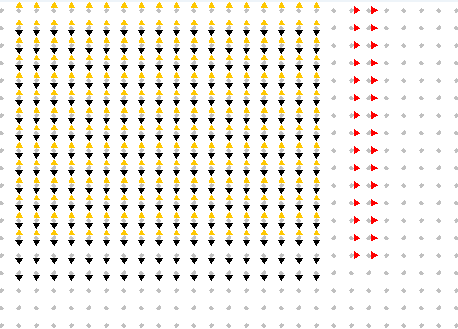
\includegraphics[width=0.49\columnwidth]{Figures/Week 5/HPP Mega Collision before.png}
    \caption{Screenshot of HPP model before particle collision}
    \label{fig:W5-hpp-before}
\end{figure}
\begin{figure}[H] 
    \centering
    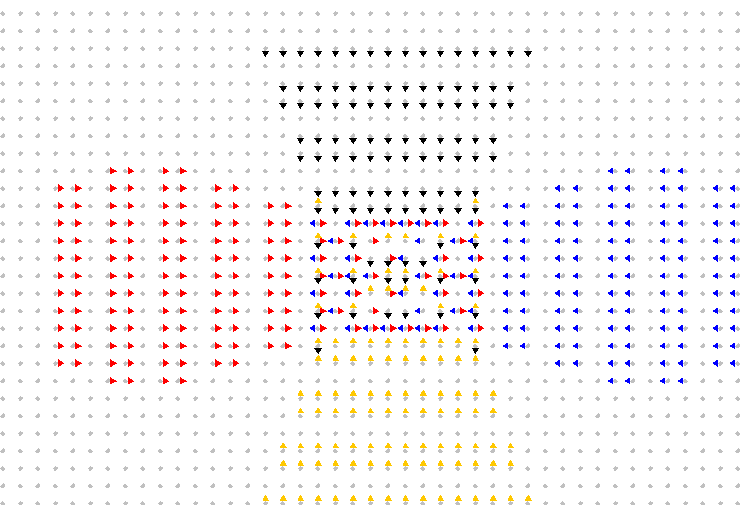
\includegraphics[width=0.49\columnwidth]{Figures/Week 5/HPP Mega Collision After.png}
    \caption{Screenshot of HPP model after particle collision}
    \label{fig:W5-hpp-after}
\end{figure}


\subsection{FHP}
An FHP model was implemented, it's more realistic than HPP and provides many more states representing the particle direction. An FHP class was provided, \autoref{fig:W5-fhp-initial} shows the initial output of the program.


\begin{figure}[H] 
    \centering
    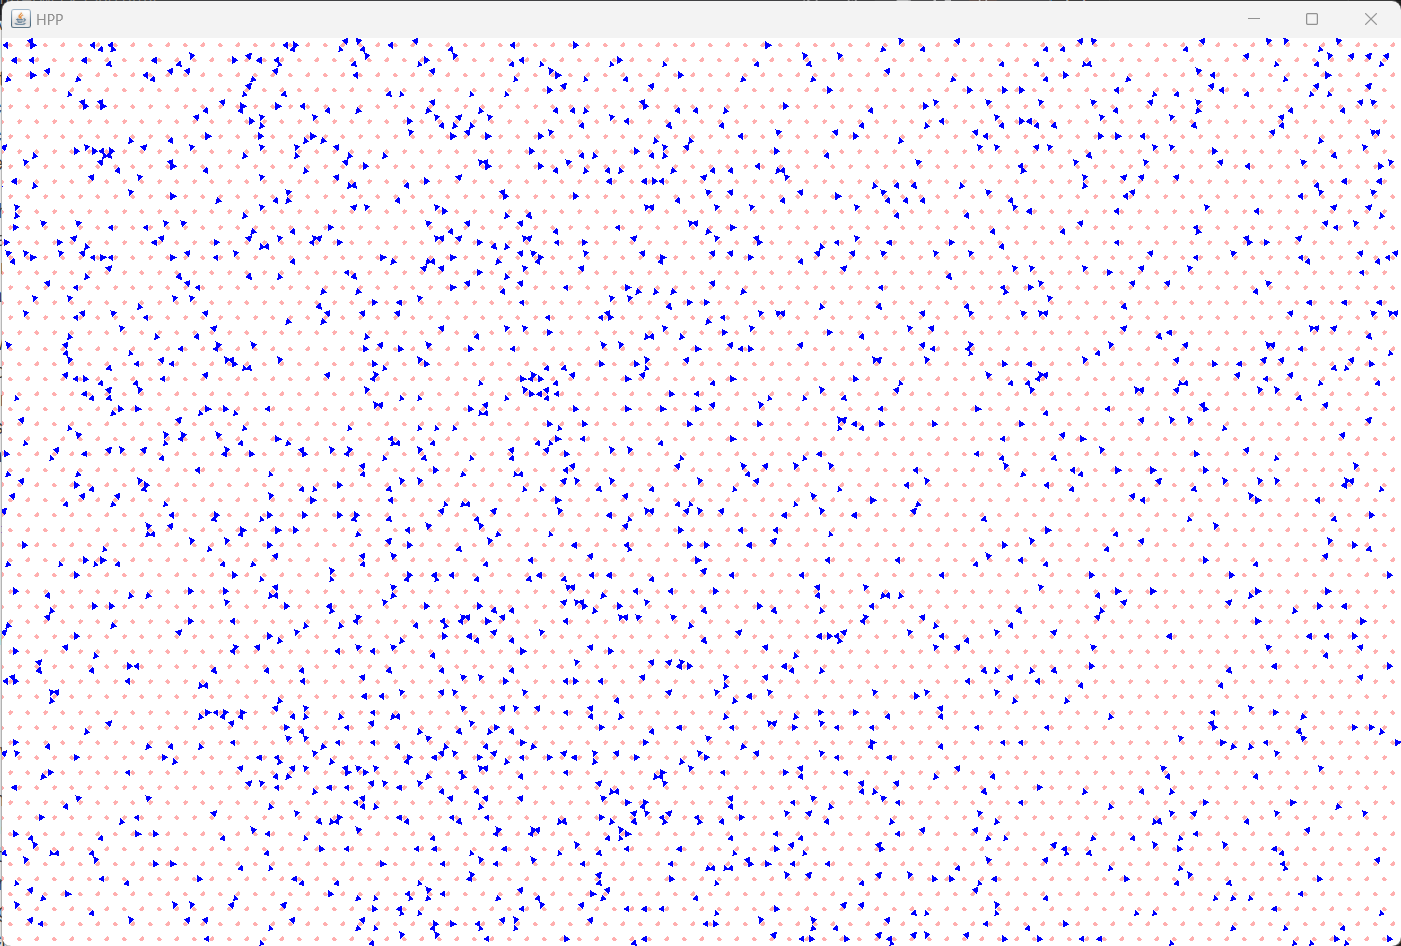
\includegraphics[width=0.9\columnwidth]{Figures/Week 5/FHP Initial Run .png}
    \caption{Screenshot of the initial FHP graphical output}
    \label{fig:W5-fhp-initial}
\end{figure}

\subsubsection{FPP Colour}
To make the particle densities clearer, a colouring scheme was implemented to set pixel colour based on particle density. The code implementing the colour setting is shown in \autoref{fig:W5-FHP-Color-code}. The program counts nearby particles 3 indexes away. Colour intensity correlates with density, the colour changes per \autoref{tab:w5-colour-table}. 

\begin{table}[htbp]
  \centering
  \renewcommand{\arraystretch}{1.2}
  \begin{tabular}{|c|c|}
    \hline
    \textbf{Colour} & \textbf{Particle Density} \\
    \hline
    Black & No particles \\
    \hline
    Green & Low Density \\
    \hline
    Yellow & Medium Density \\
    \hline
    Red & Most dense \\
    \hline
  \end{tabular}
  \caption{FHP Colours based on density}
  \label{tab:w5-colour-table}
\end{table}
.
\begin{figure}[H] 
    \centering
    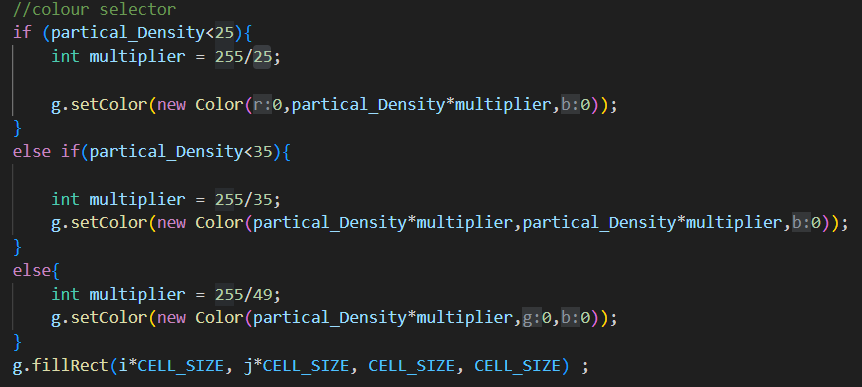
\includegraphics[width=0.9\columnwidth]{Figures/Week 5/Color/FHP Color color code.png}
    \caption{Screenshot of the FHP Colouring scheme code}
    \label{fig:W5-FHP-Color-code}
\end{figure}

\autoref{fig:W5-FHP-Color-init} shows the grid initialisation code, random particle values are set and dense circles of particles set.

\begin{figure}[H] 
    \centering
    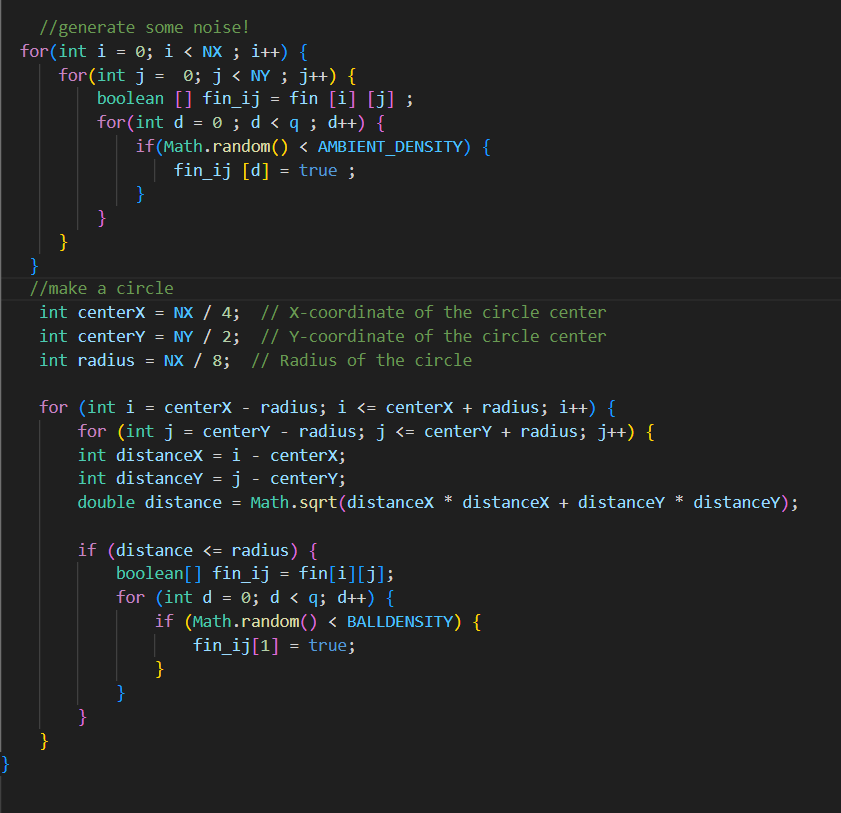
\includegraphics[width=0.9\columnwidth]{Figures/Week 5/Color/FHP color init.png}
    \caption{Screenshot of the FHP colour grid initilisation}
    \label{fig:W5-FHP-Color-init}
\end{figure}

\autoref{fig:W5-color-before} and \autoref{fig:W5-color-after} show the large balls of particles before and after collision respectively.

\begin{figure}[H] 
    \centering
    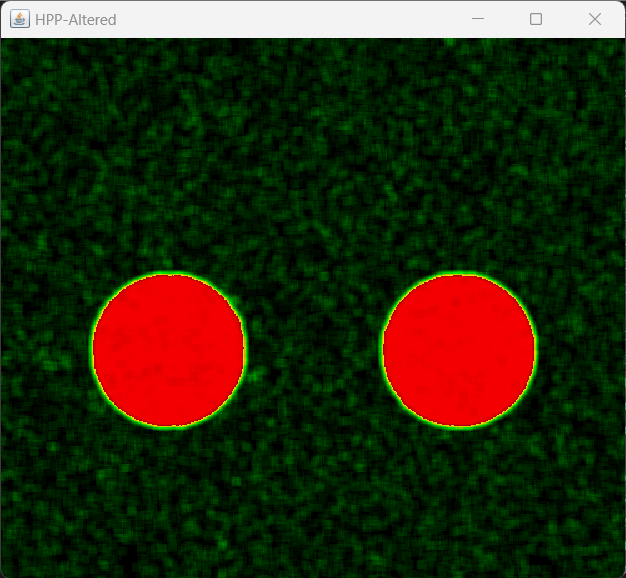
\includegraphics[width=0.49\columnwidth]{Figures/Week 5/Color/FHP Color 1.png}
    \caption{Screenshot of the FHP graphical output before collision}
    \label{fig:W5-color-before}
\end{figure}
\begin{figure}[H] 
    \centering    
    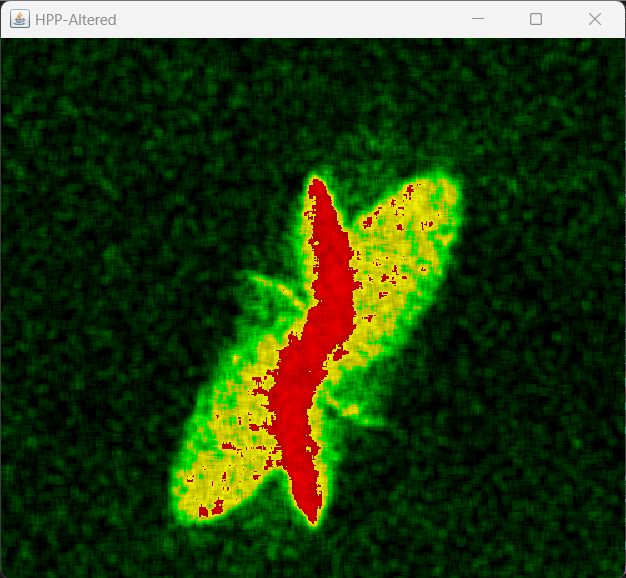
\includegraphics[width=0.49\columnwidth]{Figures/Week 5/Color/FHP Color 2.png}
    \caption{Screenshot of the FHP graphical output after collision}
    \label{fig:W5-color-after}
\end{figure}

  



\newpage
\subsubsection{FPP Large Lattice}
The previous program was extended to allow user-defined parameters \autoref{tab:FHP-large-variables}, allowing for control of how many particles are grouped together in each cell.
 \begin{table}[htbp]
      \centering
      \resizebox{1\columnwidth}{!}{\begin{tabular}{|c|c|}
    \hline
    \textbf{Varible Name} & \textbf{Usage} \\

    \hline
    Lattice{\_}Size & Defines the Lattice size \\
    \hline
    Display{\_}Size & Defines the display size, the number of particles in a group = Lattice{\_}Size/Display{\_}Size \\
    \hline
    AMBIENT{\_}Partical{\_}DENSITY & Sets the overall density of background particles\\
    \hline
    BALLDENSITY & Sets the density of particles making up the balls of particles \\
    \hline
    MAKE{\_}A{\_}VACUUM{\_}CIRCLE & Creates a circle of no particles \\
    \hline
    Color{\_}Low{\_}Cutoff & Sets the relative density for colour to change from green to yellow \\
    \hline
    Color{\_}Med{\_}Cutoff & Sets the relative density for colour to change from yellow to red \\
    \hline
  \end{tabular}}
  \caption{FHP Variable definitions}
  \label{tab:FHP-large-variables}
\end{table}

These constants are set in \autoref{fig:W5-large-lattice-var-init}.

\begin{figure}[H] 
   \centering
   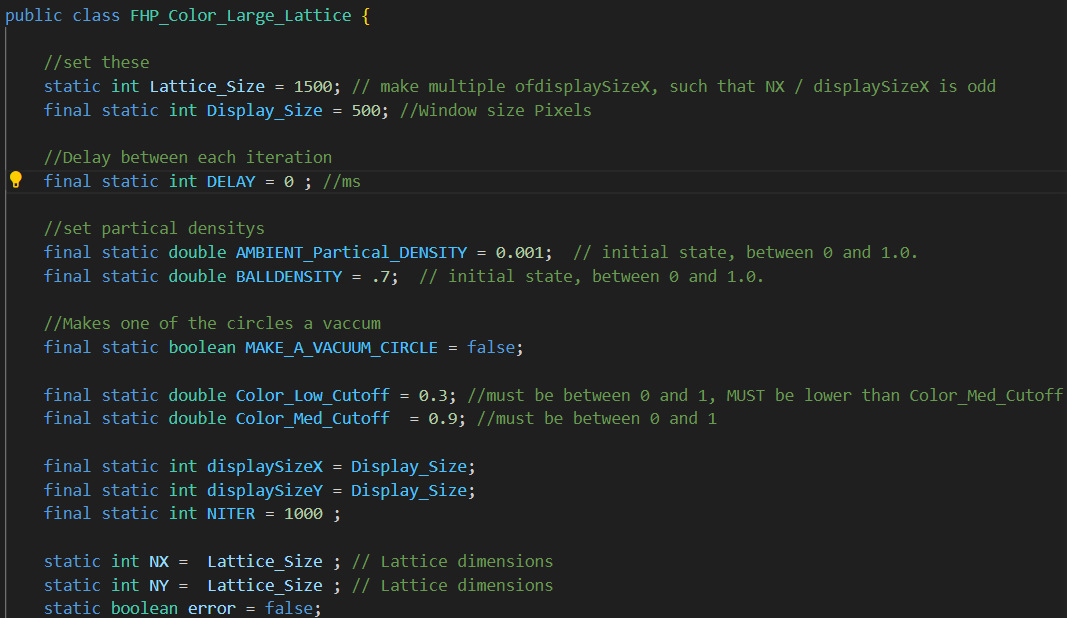
\includegraphics[width=0.9\columnwidth]{Figures/Week 5/large-lattice/FHP large-lat init.png}
   \caption{Screenshot of the FHP Large lattice constant definitions}
   \label{fig:W5-large-lattice-var-init}
\end{figure}

\autoref{fig:W5-large-lattice-validate} shows code validating that the lattice/window sizes are compatible, if not, outputs valid a lattice-size.
\begin{figure}[H] 
   \centering
   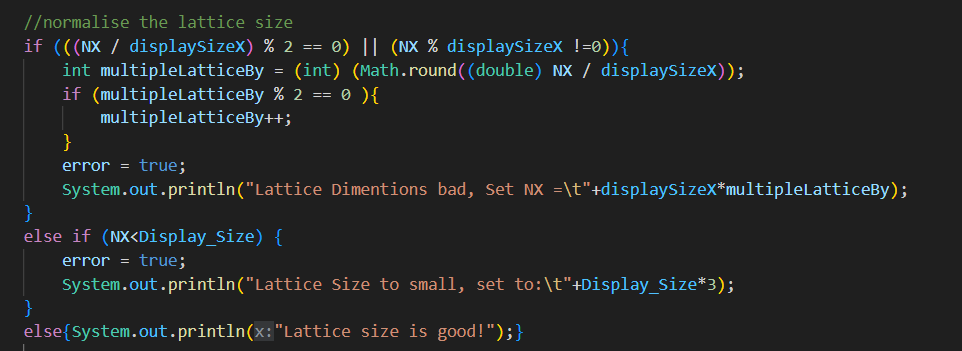
\includegraphics[width=0.9\columnwidth]{Figures/Week 5/large-lattice/FHP large-lat validate.png}
   \caption{Screenshot of the FHP Large lattice constant validation code}
   \label{fig:W5-large-lattice-validate}
\end{figure}

As the maximum number of neighbours depends on user input, the colour multipliers are calculated at runtime to ensure colour values are not $>255$ \autoref{fig:W5-large-lattice-color-multiplier}.
\begin{figure}[H] 
   \centering
   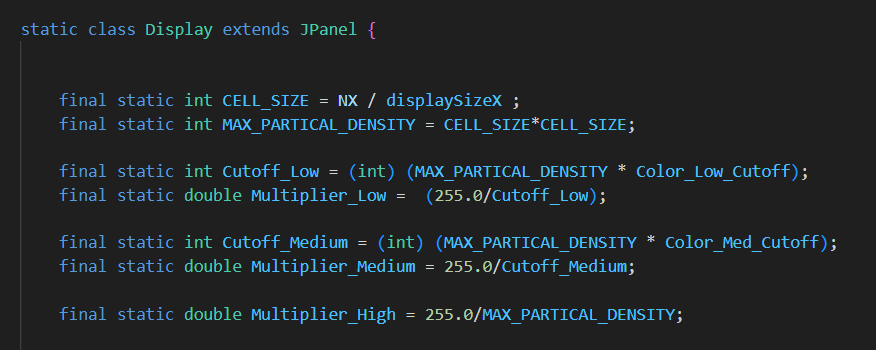
\includegraphics[width=1\columnwidth]{Figures/Week 5/large-lattice/FHP large-lat color multiplier.png}
   \caption{Screenshot of the FHP Large lattice Colour multipliers calculation code}
   \label{fig:W5-large-lattice-color-multiplier}
\end{figure}

These multipliers are used to produce a colour value for each cell, \autoref{fig:W5-large-lattice-colorer}.

\begin{figure}[H] 
   \centering
   \includegraphics[width=0.9\columnwidth]{Figures/Week 5/large-lattice/FHP large-lat color calculator.png}
   \caption{Screenshot of the FHP Large lattice Colour calculation code}
   \label{fig:W5-large-lattice-colorer}
\end{figure}

Finally, the simulation can be run, \autoref{fig:W5-large-lattice-before-collision} and \autoref{fig:W5-large-lattice-before-collision} show the simulation before and after the collision. 

\begin{figure}[H] 
   \centering
   \includegraphics[width=0.4\columnwidth]{Figures/Week 5/large-lattice/W5-before-collision.png}
   \caption{Screenshot of the FHP Large lattice, Balls before collision}
   \label{fig:W5-large-lattice-before-collision}
\end{figure}

\begin{figure}[H] 
   \centering
   \includegraphics[width=0.4\columnwidth]{Figures/Week 5/large-lattice/W5-after-collision.png}
   \caption{Screenshot of the FHP Large lattice, Balls after collision}
   \label{fig:W5-large-lattice-after-collision}
\end{figure}




\subsubsection{Vacuum}
\autoref{fig:W5-large-lattice-init-vac} shows code which creates a vacuum in the lattice.
\begin{figure}[H] 
   \centering
   \includegraphics[width=0.9\columnwidth]{Figures/Week 5/large-lattice/FHP large-lat make vaccum.png}
   \caption{Screenshot of the FHP Large lattice code which creates a vacuum}
   \label{fig:W5-large-lattice-init-vac}
\end{figure}

\autoref{fig:W5-large-lattice-vac-start} and \autoref{fig:W5-large-lattice-vac-end} shows the surrounding particles converge on the vacuum, causing the vacuum to collapse. 

\begin{figure}[H] 
   \centering
   \includegraphics[width=0.49\columnwidth]{Figures/Week 5/large-lattice/W5-vac-before-collision.png}
   \caption{Screenshot of the FHP Large lattice vacuum sphere simulation before collapse}
   \label{fig:W5-large-lattice-vac-start}
\end{figure}

\begin{figure}[H] 
   \centering
   \includegraphics[width=0.49\columnwidth]{Figures/Week 5/large-lattice/W5-vac-after-collision.png}
   \caption{Screenshot of the FHP Large lattice vacuum sphere simulation after collapse}
   \label{fig:W5-large-lattice-vac-end}
\end{figure}



\newpage
\section{Lab 6 - Excitable Media} 
Excitable media are a class of systems which propagate waves which form repeating patterns, these waves are by local disturbances and are sustained. Applications for such systems are widespread, a notable example is heart monitoring. These systems do not allow a wave to propagate for a set period of time, this is a 'resting' state.


\subsection{3 State CA}
A three-state CA was used to simulate repeating waves. The initial spiral wave output is shown in figure \autoref{fig:W6-initial-3CA}.

\begin{figure}[H] 
    \centering
    \includegraphics[width=0.49\columnwidth]{Figures/Week 6/3stateCA-Initial.png}
    \caption{Screenshot of the graphical output of the initial 3-state CA}
    \label{fig:W6-initial-3CA}
\end{figure}

The Java code was altered to allow for a plane wave simulation. To achieve this, the nested for loop which breaks the initial wave was removed. To allow the wave to repeat itself, the state of all indices on the bottom half of the 'state' matrix was set to '0'. The code and output of the program are shown in Figures \ref{fig:W6-3CA-plane-code} and \ref{fig:W6-3CA-plane-output}. 


\begin{figure}[H] 
    \centering
    \includegraphics[width=0.49\columnwidth]{Figures/Week 6/3stateCA-plane-code.png}
    \caption{Screenshot of the Java code to produce a plane wave}
    \label{fig:W6-3CA-plane-code}
\end{figure}

\begin{figure}[H] 
    \centering
    \includegraphics[width=0.49\columnwidth]{Figures/Week 6/3stateCA-plane-output.png}
    \caption{Screenshot of the graphical output of a plane wave using 3-state CA}
    \label{fig:W6-3CA-plane-output}
\end{figure}



To allow different starting locations, branching was implemented to set the starting location and wave type. Variable 'startLocation' must be set to '1', '2' or'3' to define the starting location. \autoref{fig:W6-3CA-conditional-logic-code} shows the code implementing this.

A similar approach was created to allow the user to define the 'doSpiralWave' variable, allowing the wave type to be altered.

\begin{figure}[H] 
    \centering
    \includegraphics[width=0.6\columnwidth]{Figures/Week 6/3stateCA-plane-logic-code.png}
    \caption{Screenshot of the code controlling simulation start-location logic}
    \label{fig:W6-3CA-conditional-logic-code}
\end{figure}

\newpage

\autoref{fig:W6-3CA-start-corner} shows the graphical output when 'startLocation=3', starting the simulation in the corner of the grid. It sets all the 'state' array values to '0', with the exception of a small box of excited cells in one corner.

\begin{figure}[H] 
    \centering
    \includegraphics[width=0.49\columnwidth]{Figures/Week 6/3stateCA-CORNER-output.png}
    \caption{Screenshot of 3-State CA simulation starting in the corner of the grid}
    \label{fig:W6-3CA-start-corner}
\end{figure}

\autoref{fig:W6-3CA-start-middle} shows the graphical output when 'startLocation=2', starting the simulation in the centre. 
\begin{figure}[H] 
    \centering
    \includegraphics[width=0.49\columnwidth]{Figures/Week 6/3stateCA-MIDDLE-output.png}
    \caption{Screenshot of 3-State CA simulation starting in the middle of the grid}
    \label{fig:W6-3CA-start-middle}
\end{figure}

\subsection{GST}
A Gerhardt-Schuster-Tyson model was implemented to create a spiral and plane wave. The highlighted nested for loop shown in \autoref{fig:W6-GST-plane-code} was removed to create a plane wave simulation. \autoref{fig:W6-GST-side-by-side-output} shows both spiral (left side) and plane wave (right side) simulation outputs.

\begin{figure}[H] 
    \centering
    \includegraphics[width=0.49\columnwidth]{Figures/Week 6/GST-plane-code.png}
    \caption{Screenshot of the GST plane wave code alteration}
    \label{fig:W6-GST-plane-code}
\end{figure}

\begin{figure}[H] 
    \centering
    \includegraphics[width=0.49\columnwidth]{Figures/Week 6/GST-side-by-side-output.png}
    \caption{Screenshot of the graphical output of GST spiral (left) and plane (right) wave simulations}
    \label{fig:W6-GST-side-by-side-output}
\end{figure}


Changing the value of some parameters alters the wave shape, size and stability. For instance, increasing the value of 'K0\_EXCI' to '10' decreases cell excitability. This causes the wave formation to look square, rather than circular, in addition to reducing the width of the wave and slowing the wave propagation speed. This is shown in \autoref{fig:W6-GST-less-excitable}.

\begin{figure}[H] 
    \centering
    \includegraphics[width=0.49\columnwidth]{Figures/Week 6/gst-square.png}
    \caption{Screenshot of the graphical output of GST when cell excitability is reduced}
    \label{fig:W6-GST-less-excitable}
\end{figure}


Altering the 'K0\_RECO' sets the minimum number of unexcited neighbours to set a cell's state to recovery. Increasing the value causes more cells to remain excited after each wave has passed, these cells usually appear near the edges of the matrix, introducing 'noise' into the system. \autoref{fig:W6-GST-high-min-neighbours} shows these pixels at the edges of the grid.


Inversely, reducing this value decreases the number of cells left excited after a wave has passed, seen in \autoref{fig:W6-GST-low-min-neighbours}.
\begin{figure}[H] 
    \centering
    \includegraphics[width=0.49\columnwidth]{Figures/Week 6/GST-high-min-neighbours.png}
    \caption{Screenshot of the graphical output of GST when K0\_RECO is high}
    \label{fig:W6-GST-high-min-neighbours}
\end{figure}

\begin{figure}[H] 
    \centering
    \includegraphics[width=0.49\columnwidth]{Figures/Week 6/GST-low-min-neighbours.png}
    \caption{Screenshot of the graphical output of GST when K0\_RECO is low}
    \label{fig:W6-GST-low-min-neighbours}
\end{figure}

The neighbourhood radius correlates with the width of the wave, increasing this value causes the wave to be thicker \autoref{fig:W6-GST-high-radius}. The origin of the spiral become lower on the grid with higher values.

\begin{figure}[H] 
    \centering
    \includegraphics[width=0.49\columnwidth]{Figures/Week 6/GST-Large-Radius.png}
    \caption{Screenshot of the graphical output of GST when 'R' - radius is increased}
    \label{fig:W6-GST-high-radius}
\end{figure}
\newpage
\subsection{4 State CA}
The initial three-state CA was built upon to add another excited state, state '3' now represents the front of a wave. In addition to the extra state, another array timeToStateChange was created to store the time value until a state may change. \autoref{fig:W6-4CA-dec} shows the variable declaration, \autoref{fig:W6-4CA-init} shows the arrays' value initiation.


\begin{figure}[H] 
    \centering
    \includegraphics[width=1\columnwidth]{Figures/Week 6/4stateCA-time-delaration.png}
    \caption{Screenshot of the 'timeToStateChange' declaration code}
    \label{fig:W6-4CA-dec}
\end{figure}

\begin{figure}[H] 
    \centering
    \includegraphics[width=1\columnwidth]{Figures/Week 6/4stateCA-time-values-init.png}
    \caption{Screenshot of the 'timeToStateChange' initiation code}
    \label{fig:W6-4CA-init}
\end{figure}


The timeToStateChange stores an integer between 0 and 3. In each iteration, all time values are decremented towards 0. This value is updated each state change to the corresponding value in \autoref{tab:state-time-values}.

\begin{table}[htbp]
  \centering
  \renewcommand{\arraystretch}{1.2}
  \begin{tabular}{|c|c|}
    \hline
    \textbf{state} & \textbf{timeToStateChange} \\

    \hline
    1 & 3 \\
    \hline
    2 & 3 \\
    \hline
    3 & 2 \\
    \hline
  \end{tabular}
  \caption{timeToStateChange value when a cell transitions into each state}
  \label{tab:state-time-values}
\end{table}


The program must search for excited neighbours. The neighbour radius has been increased by four to eight neighbours, meaning cells which are diagonally adjacent to the origin cells are included in the search. \autoref{fig:W6-4CA-search-code} Shows that two comparisons are made on each of these cell - setting excitedNeighbour to true, if either a '2' or '3' is found in any of the eight cells. 
\begin{figure}[H] 
    \centering
    \includegraphics[width=1\columnwidth]{Figures/Week 6/4stateCA-neighbour-search-code.png}
    \caption{Screenshot of 'fourStateCA' code searching for excited neighbours}
    \label{fig:W6-4CA-search-code}
\end{figure}

In each iteration, the program must update each 'state' and 'timeToStateChange' value. The first conditional statement, shown in \autoref{fig:W6-4CA-search-code}, decrements the 'timeToStateChange' by one. 

After this the switch statement updates the 'state' and 'timeToStateChange' values dependant on if the cell has excited neighbours or not, and if timeToStateChange is 0.  

\begin{figure}[H] 
    \centering
    \includegraphics[width=1\columnwidth]{Figures/Week 6/4stateCA-update-code.png}
    \caption{Screenshot of fourStateCA Code updating 'state' and 'timeToStateChange' arrays}
    \label{fig:W6-4CA-update-code}
\end{figure}


\autoref{fig:W6-4CA-colour-code} shows an additional colouring condition has been added, allowing a different colour for the new state=3, the colouring scheme is outlined in \autoref{tab:state-color-values}.  

\begin{figure}[H] 
    \centering
    \includegraphics[width=1\columnwidth]{Figures/Week 6/4stateCA-color-code.png}
    \caption{Screenshot of fourStateCA cell colouring code}
    \label{fig:W6-4CA-colour-code}
\end{figure}

\vspace{10mm}
\begin{table}[htbp]
  \centering
  \begin{tabular}{|c|c|c|}
    \hline
    \textbf{State Number} &\textbf{State Meaning} & \textbf{Cell Colour} \\

    \hline
    0 & Resting & Background (White)\\
    \hline
    1 & Recovering & Blue \\
    \hline
    2 & Excited-Wave-Plateau & Dark Red \\
    \hline
    3 & Excited-Wave-Front & Bright Red \\
    \hline
  \end{tabular}
  \caption{'fourStateCA' Cell Colour Scheme}
  \label{tab:state-color-values}
\end{table}

The graphical output for the program is shown in \autoref{fig:W6-4CA-output}.
\begin{figure}[H] 
    \centering
    \includegraphics[width=0.49\columnwidth]{Figures/Week 6/4stateCA-output.png}
    \caption{Screenshot of 'fourStateCA' graphical output}
    \label{fig:W6-4CA-output}
\end{figure}

\newpage

\section{Lab 7 - Lattice Boltzmann Model}
LBM models are similar to the previously discusses FHP and HPP models, however, it has a greater focus on the statistical mechanics of molecules. The model utilises probability distributions based on Boltzmann's equation \autoref{fig:boltzmann}, in particular, the distribution of individual molecules having a certain position or velocity. Function $f$ gives a continuous range, this differs from the Boolean value used in the FHP model, thus when discretised - the output array should have floating point elements. 

Local density in LBM is the sum of the local velocity states, and local velocity is a weighted average of discrete flow velocities. 
    \begin{center}
        \begin{equation}
           \frac{\partial f}{\partial t} + v \cdot \nabla f + g \cdot \frac{\partial f}{\partial v} = \omega(f)
            \label{fig:boltzmann}
        \end{equation}  
    \end{center}%Equation

\autoref{fig:W10-lbm-5000} shows the flow of fluid quickly causes vortices behind the obstacle when run. 


\begin{figure}[H] 
    \centering
    \includegraphics[width=0.49\columnwidth]{Figures/Week 7/LBM-Initial-5000-iterations-output.png}
    \caption{Screenshot of the graphical output LBM 5000 iterations}
    \label{fig:W10-lbm-5000}
\end{figure}

Loop unrolling improved performance, the benchmarking results are shown in \autoref{fig:W7-bench-results-table} and \autoref{fig:W7-Graph}.

On average the program ran $111499.3333 / 60259.33333= 1.850324708$ times faster, this is a massive speedup.
\begin{table}[htbp]
      \centering
      \begin{tabular}{|c|c|c|}
            \hline
            \textbf{Run Number} &\textbf{Unrolled Loop} & \textbf{Rolled Loop} \\
            \hline
            Run 1 & 64319 & 119067 \\
            \hline
            Run 2 & 61434 & 101983 \\
            \hline
            Run 3 & 55025 & 113448 \\
            \hline
            Mean & 60259.33333 & 111499.3333 \\
            \hline                      
      \end{tabular}
      \caption{Lab 10 LBM Benchmarking Results}
      \label{fig:W7-bench-results-table}
    \end{table}  
\begin{figure}[H] 
    \centering
    \includegraphics[width=0.9\columnwidth]{Figures/Week 7/graph.png}
    \caption{LBM unrolled loop results graph}
    \label{fig:W7-Graph}
\end{figure}

\autoref{fig:W7-lbm-30000} shows that by iteration 15000 (top) the vortices have left a 'Von Karman vortex street' (VKVS) behind the obstacle and by 30000 (bottom) the trail is well established.

\begin{figure}[H] 
    \centering
    \includegraphics[width=0.49\columnwidth]{Figures/Week 7/LBM-Initial-15000-30000-iterations-output.png}
    \caption{Screenshot of the graphical output LBM 30000 iterations}
    \label{fig:W7-lbm-30000}
\end{figure}


\autoref{fig:W7-lbm-square-code} shows code implementing a square obstacle, high pressure quickly builds around each vertex before two vortices are created on the rear two vertexes \autoref{fig:W7-lbm-square-sim}  
\begin{figure}[H] 
    \centering
    \includegraphics[width=0.49\columnwidth]{Figures/Week 7/square code.png}
    \caption{Screenshot of the LMB code implementing square obstacle}
    \label{fig:W7-lbm-square-code}
\end{figure}
\begin{figure}[H] 
    \centering
    \includegraphics[width=0.49\columnwidth]{Figures/Week 7/square run.png}
    \caption{Screenshot of the LMB square obstacle simulation}
    \label{fig:W7-lbm-square-sim}
\end{figure}
\newpage
\section{Lab 8 - Aerodynamics}
This lab extends the previous LBM model by altering the boundary conditions. The system implements a no-slip condition, meaning that the fluid that collides with a boundary is assumed to be stationary. The 'bounce-back' scheme has been implemented to 'bounce' particles in the same direction that came from when they collide with a boundary.   

The Reynolds Number is a quantity used to characterise flow, it's used to determine the type of flow in the simulation. 
\[\mathrm{Re} = \mathbf{|u|}  \mathbf{L} \mathbf{/V}\]
where $|u|$ is a charactistic of the flow velocity, $L$ is the length of an obstacle and $v$ is viscosity.
Lower Reynolds values are associated with turbulent flow and high with laminar. 

The obstacle in the simulation is an airfoil. When the first fluid passes the obstacle, a pressure wave is visible propagating through the system \autoref{fig:W8-1}.
\begin{figure}[H] 
    \centering
    \includegraphics[width=0.6\columnwidth]{Figures/Week 8/1.png}
    \caption{Screenshot of the Airfoil simulation, pressure wave on left}
    \label{fig:W8-1}
\end{figure}
Soon, the fluid reaches the outlet and bounces back. This is seen in \autoref{fig:W8-bounceback}.
\begin{figure}[H]   
    \centering
    \includegraphics[width=0.49\columnwidth]{Figures/Week 8/bounceback.png}
    \caption{Screenshot of the LBM Airfoil bounce-back}
    \label{fig:W8-bounceback}
\end{figure}
\autoref{fig:W8-trail} shows as the simulation continues, another VKVS trail is visible, although with lower amplitude oscillations than previously, due to the aerodynamic shape of the Airfoil.
\begin{figure}[H] 
    \centering
    \includegraphics[width=0.49\columnwidth]{Figures/Week 8/trail.png}
    \caption{Screenshot of the LMB Airfoil trail}
    \label{fig:W8-trail}
\end{figure}

\autoref{fig:W8-cli-1} shows the lift and drag values the airfoil experiences are 0.01 and 0.03 respectively.
\begin{figure}[H] 
    \centering
    \includegraphics[width=0.49\columnwidth]{Figures/Week 8/cli.png}
    \caption{Screenshot of the console output from LBM Airfoil }
    \label{fig:W8-cli-1}
\end{figure}

Increasing the Alpha variable to '10' causes the airfoil angle of attack to be greater \autoref{fig:W8-alphga-10}. The increase in drag is small, however, the lift increased to 0.07 - this is a massive increase \autoref{fig:W8-alphga-20}.

\begin{figure}[H] 
    \centering
    \includegraphics[width=0.49\columnwidth]{Figures/Week 8/alpha 10 1.png}
    \caption{Screenshot of the LBM Airfoil high alpha value}
    \label{fig:W8-alphga-10}
\end{figure}
\begin{figure}[H] 
    \centering
    \includegraphics[width=0.49\columnwidth]{Figures/Week 8/alpha 10 1.png}
    \caption{Screenshot of the LBM Airfoil high alpha value}
    \label{fig:W8-alphga-20}
\end{figure}


Inversely, setting alpha to -10 causes the lift to become negative, this would cause the airfoil to descend. \autoref{fig:W8-alphga-minus-output} shows the simulation and the negative lift in \autoref{fig:W8-alphga-minus-cli}, interestingly, the horizontal drag value isn't impacted. 
\begin{figure}[H] 
    \centering
    \includegraphics[width=0.49\columnwidth]{Figures/Week 8/neg sim.png}
    \caption{Screenshot of the LBM Airfoil with negative alpha value}
    \label{fig:W8-alphga-minus-output}
\end{figure}
\begin{figure}[H] 
    \centering
    \includegraphics[width=0.49\columnwidth]{Figures/Week 8/neg cli.png}
    \caption{Screenshot of the LBM Airfoil console with negative alpha value }
    \label{fig:W8-alphga-minus-cli}
\end{figure}


\newpage
\section{Lab 10 - Differential Equations}
A Python script which calculates the motion between two bodies with mass and gravitational force. The 'scipy.integrate.solve{\_}ivp' method is used to solve initial value problems using the Runge-Kutta method, here solving for Newton's equations of motion for the bodies. A function 'fun' is passed to the method, it is a system of ordinary differential equations. A function called 'grav' is used in these calculations, it calculates the inverse-square-law between the two particles. \autoref{fig:W10-1} shows the output for the program, an animation of the two particles orbiting each other. Eventually, the orbits begin to decay.

\begin{figure}[H] 
    \centering
    \includegraphics[width=0.49\columnwidth]{Figures/Week 10/1.png}
    \caption{Screenshot of the initial Python Runge-Kutta method output}
    \label{fig:W10-1}
\end{figure}

The Leapfrog method was implemented to solve the equations, it is similar to Euler method, except velocities are defined for 1/2 integer steps, the output of this program is shown in \autoref{fig:W10-2}. In this simulation, the orbit does not decay as it did with the Runge-Kutta implementation.
\begin{figure}[H] 
    \centering
    \includegraphics[width=0.49\columnwidth]{Figures/Week 10/2.png}
    \caption{Screenshot of the Python Leapfrog method output}
    \label{fig:W10-2}
\end{figure}

The value of 'dt' was set to 0.1, increasing the step size. This causes the particles to fly out of the simulation \autoref{fig:W10-3} as the orbit grows.
\begin{figure}[H] 
    \centering
    \includegraphics[width=0.49\columnwidth]{Figures/Week 10/3.png}
    \caption{Screenshot of the Python Leapfrog method dt=0.1}
    \label{fig:W10-3}
\end{figure}

When the value is set to 0.005, the program takes twice as long to execute due to the increased number of steps to calculate. The orbit is smaller than it was previously \autoref{fig:W10-4}.


\begin{figure}[H] 
    \centering
    \includegraphics[width=0.49\columnwidth]{Figures/Week 10/4.png}
    \caption{Screenshot of the Python Leapfrog method dt=0.005}
    \label{fig:W10-4}
\end{figure}

Increasing the initial values of 't'/'tend' cause the speed of the orbit to slow dramatically \autoref{fig:W10-5}.
\begin{figure}[H] 
    \centering
    \includegraphics[width=0.49\columnwidth]{Figures/Week 10/5.png}
    \caption{Screenshot of the Python Leapfrog method Increased initial values}
    \label{fig:W10-5}
\end{figure}
\newpage



